%-----------------------------------------------------------------------------
%
%               Template for sigplanconf LaTeX Class
%
% Name:         sigplanconf-template.tex
%
% Purpose:      A template for sigplanconf.cls, which is a LaTeX 2e class
%               file for SIGPLAN conference proceedings.
%
% Guide:        Refer to "Author's Guide to the ACM SIGPLAN Class,"
%               sigplanconf-guide.pdf
%
% Author:       Paul C. Anagnostopoulos
%               Windfall Software
%               978 371-2316
%               paul@windfall.com
%
% Created:      15 February 2005
%
%-----------------------------------------------------------------------------


\documentclass[10pt]{sigplanconf}
\usepackage{todonotes}

% The following \documentclass options may be useful:

% preprint      Remove this option only once the paper is in final form.
% 10pt          To set in 10-point type instead of 9-point.
% 11pt          To set in 11-point type instead of 9-point.
% numbers       To obtain numeric citation style instead of author/year.

\usepackage{amsmath}
\usepackage{amsthm}
\usepackage{amssymb}
\usepackage{bcprules}
\usepackage{prooftree}
\usepackage{multicol}
\usepackage{mathpartir}
\usepackage{listings}
\usepackage{xspace}
\usepackage{mdframed}
\usepackage{xcolor}
\usepackage{fontspec}
\usepackage{graphicx}
\usepackage{setspace}
\usepackage{wasysym}
\usepackage{url}
\usepackage{caption}
\usepackage{subcaption}
\usepackage{csquotes}
\usepackage{enumitem}

\usepackage{balance}


\makeatletter
\def \@ivtitleauthors#1#2#3#4{%
  \if \@andp{\@emptyargp{#2}}{\@emptyargp{#3}}%
    \noindent \@setauthor{40pc}{#1}{\@false}\par
  \else\if \@emptyargp{#3}%
    \noindent \@setauthor{17pc}{#1}{\@false}\hspace{3pc}%
              \@setauthor{17pc}{#2}{\@false}\par
  \else\if \@emptyargp{#4}%
    \noindent \@setauthor{17pc}{#1}{\@false}\hspace{3pc}%
              \@setauthor{17pc}{#3}{\@false}\par
  \else
    \noindent \@setauthor{9.3333pc}{#1}{\@false}\hspace{1.5pc}%
              \@setauthor{9.3333pc}{#2}{\@false}\hspace{1.5pc}%
              \@setauthor{9.3333pc}{#3}{\@false}\hspace{1.5pc}%
              \@setauthor{9.3333pc}{#4}{\@true}\par
    \relax
  \fi\fi\fi
  \vspace{20pt}}
\def \@maketitle {%
  \begin{center}
  \@settitlebanner
  \let \thanks = \titlenote
  {\leftskip = 0pt plus 0.25\linewidth
   \rightskip = 0pt plus 0.25 \linewidth
   \parfillskip = 0pt
   \spaceskip = .7em
   \noindent \LARGE \bfseries \@titletext \par}
  \vskip 6pt
  \noindent \Large \@subtitletext \par
  \vskip 12pt
  \ifcase \@authorcount
    \@latex@error{No authors were specified for this paper}{}\or
    \@titleauthors{i}{}{}\or
    \@titleauthors{i}{ii}{}\or
    \@titleauthors{i}{ii}{iii}\or
    \@ivtitleauthors{i}{ii}{iii}{iv}\or
    \@titleauthors{i}{ii}{iii}\@titleauthors{iv}{v}{}\or
    \@titleauthors{i}{ii}{iii}\@titleauthors{iv}{v}{vi}\or
    \@titleauthors{i}{ii}{iii}\@titleauthors{iv}{v}{vi}%
                  \@titleauthors{vii}{}{}\or
    \@titleauthors{i}{ii}{iii}\@titleauthors{iv}{v}{vi}%
                  \@titleauthors{vii}{viii}{}\or
    \@titleauthors{i}{ii}{iii}\@titleauthors{iv}{v}{vi}%
                  \@titleauthors{vii}{viii}{ix}\or
    \@titleauthors{i}{ii}{iii}\@titleauthors{iv}{v}{vi}%
                  \@titleauthors{vii}{viii}{ix}\@titleauthors{x}{}{}\or
    \@titleauthors{i}{ii}{iii}\@titleauthors{iv}{v}{vi}%
                  \@titleauthors{vii}{viii}{ix}\@titleauthors{x}{xi}{}\or
    \@titleauthors{i}{ii}{iii}\@titleauthors{iv}{v}{vi}%
                  \@titleauthors{vii}{viii}{ix}\@titleauthors{x}{xi}{xii}%
  \else
    \@latex@error{Cannot handle more than 12 authors}{}%
  \fi
  \vspace{1.75pc}
  \end{center}}
\makeatother


%%%%%%%%%%%%%%%%%%%%%%%%%%%%%%%%%%%%%%%
%   General                           %
%%%%%%%%%%%%%%%%%%%%%%%%%%%%%%%%%%%%%%%

\lstdefinelanguage{Scala}%
{morekeywords={abstract,case,catch,char,class,%
    def,else,extends,final,%
    if,import,%
    match,module,new,null,object,override,package,private,protected,%
    public,return,super,this,throw,trait,try,type,val,var,with,implicit,%
    macro,sealed,%
  },%
  sensitive,%
  morecomment=[l]//,%
  morecomment=[s]{/*}{*/},%
  morestring=[b]",%
  morestring=[b]',%
  showstringspaces=false%
}[keywords,comments,strings]%

\lstset{language=Scala,%
  mathescape=true,%
  columns=[c]fixed,%
  basewidth={0.5em, 0.40em},%
  basicstyle=\tt,%
  commentstyle=\color{gray}\itshape\ttfamily,
  xleftmargin=0.0cm
}
% \lstset{tabsize=2,
% basicstyle=\ttfamily\fontsize{9pt}{1em}\selectfont,
% commentstyle=\color{gray}\itshape\ttfamily,
% numbers=left, numberstyle=\scriptsize\color{gray}\ttfamily, language=scala,moredelim=[il][\sffamily]{?},mathescape=false,showspaces=false,showstringspaces=false,xleftmargin=15pt,escapechar=@, morekeywords=[1]{let,fn,val},deletekeywords={for},classoffset=0,belowskip=\smallskipamount
% }

\theoremstyle{definition}
\newmdtheoremenv[hidealllines=true,topline=true,bottomline=true,skipabove=\baselineskip,skipbelow=\baselineskip]{defn}{Definition}[section]
\theoremstyle{definition}
\newmdtheoremenv[hidealllines=true,topline=true,bottomline=true,skipabove=\baselineskip,skipbelow=\baselineskip]{prop}{Property}[section]
% \theoremstyle{nonumberplain}
% \theoremstyle{definition}
% \newmdtheoremenv*[hidealllines=true,topline=true,bottomline=true,skipabove=\baselineskip,skipbelow=\baselineskip]{defnn}{Definition}[section]
\newtheorem*{defn*}{Definition}
% \newtheorem{defn}{Definition}[section]
% \newenvironment{defn}
  % {\begin{mdframed}[style=warning]\begin{mdef}}
  % {\end{mdef}\end{mdframed}}

% Comments and notes
\newcommand{\comment}[1]{}
\newcommand{\note}[1]{{\bf $\clubsuit$ #1 $\spadesuit$}}
\newcommand{\ifreport}[1]{#1}
%\newcommand{\ifreport}[1]{}

% Abbreviations and emphasis
\newcommand{\ie}{{\em i.e.,~}}
\newcommand{\eg}{{\em e.g.,~}}
\newcommand{\term}[1]{\mbox{\texttt{#1}}}
\newcommand{\itl}[1]{\mbox{\textit{#1}}}

% Commas and semicolons
\newcommand{\comma}{,\,}
\newcommand{\commadots}{\comma \ldots \comma}
\newcommand{\semi}{;\mbox{;};}
\newcommand{\semidots}{\semi \ldots \semi}

% Spacing
\newcommand{\gap}{\quad\quad}
\newcommand{\biggap}{\quad\quad\quad}
\newcommand{\nextline}{\\ \\}
\newcommand{\htabwidth}{0.5cm}
\newcommand{\tabwidth}{1cm}
\newcommand{\htab}{\hspace{\htabwidth}}
\newcommand{\tab}{\hspace{\tabwidth}}
\newcommand{\linesep}{\ \hrulefill \ \smallskip}

\newcommand{\sectionline}{%
  \nointerlineskip \vspace{\baselineskip}%
  \hspace{\fill}\rule{0.5\linewidth}{.7pt}\hspace{\fill}%
  \par\nointerlineskip \vspace{\baselineskip}
}

% Figures
\newcommand{\figurebox}[1]
        {\fbox{\begin{minipage}{\textwidth} #1 \medskip\end{minipage}}}
\newcommand{\twofig}[3]
        {\begin{figure*}[t]#3\ \hrulefill\
        \caption{\label{#1}#2}\end{figure*}}
\newcommand{\boxfig}[3]
        {\begin{figure*}\figurebox{#3\caption{\label{#1}#2}}\end{figure*}}
\newcommand{\figref}[1]
        {Figure~\ref{#1}}

% Arrays
\newcommand{\ba}{\begin{array}}
\newcommand{\ea}{\end{array}}
\newcommand{\bda}{\[\ba}
\newcommand{\eda}{\ea\]}
\newcommand{\ei}{\end{array}}
\newcommand{\bcases}{\left\{\begin{array}{ll}}
\newcommand{\ecases}{\end{array}\right.}

%%%%%%%%%%%%%%%%%%%%%%%%%%%%%%%%%%%%%%%
%   Language abstraction commands     %
%%%%%%%%%%%%%%%%%%%%%%%%%%%%%%%%%%%%%%%

%% Relations
% Subtype
\newcommand{\sub}{<:}
% Type assignment
\newcommand{\typ}{:}
% Reduction
\newcommand{\reduces}{\;\rightarrow\;}
% Well-formedness
\newcommand{\wf}{\;\mbox{\textbf{wf}}}

%% Operators
% Type selection
\newcommand{\tsel}{\#}
% Function type
\newcommand{\tfun}{\rightarrow}
\newcommand{\dfun}[3]{(#1\!:\!#2) \Rightarrow #3}
% Conjunction
\newcommand{\tand}{\wedge}
% Disjunction
\newcommand{\tor}{\vee}
% Singleton type suffix
\newcommand{\sing}{.\textbf{type}}

%% Syntax
% Header for typing rules
\newcommand{\judgement}[2]{{\bf #1} \hfill \fbox{#2}}
% Refinement
\newcommand{\refine}[2]{\left\{#1 \Rightarrow #2 \right\}}
% Field definitions
\newcommand{\ldefs}[1]{\left\{#1\right\}}
% Member sequences
\newcommand{\seq}[1]{\overline{#1}}
% Lambda
\newcommand{\dabs}[3]{(#1\!:\!#2)\Rightarrow #3}
\newcommand{\abs}[3]{\lambda #1\!:\!#2.#3}
% Application
\newcommand{\app}[2]{#1\;#2}
% Substitution
\newcommand{\subst}[3]{[#1/#2]#3}
% Object creation
\newcommand{\new}[3]{\textbf{val }#1 = \textbf{new }#2 ;\; #3}
%\renewcommand{\new}[3]{#1 \leftarrow #2 \,\textbf{in}\, #3}
% Field declaration
\newcommand{\Ldecl}[3]{#1 \typ #2..#3}%{#1 \operatorname{>:} #2 \operatorname{<:} #3}
\newcommand{\ldecl}[2]{#1 \typ #2}
% Top and Bottom
\newcommand{\Top}{\top}%{\textbf{Top}}
\newcommand{\Bot}{\bot}%\textbf{Bot}}
% Environment extension
\newcommand{\envplus}[1]{\uplus \{ #1 \}}

\newcommand{\reduction}[4]{#1, #2 \reduces #3, #4}
\newcommand{\reducebig}[6]{#1, #2, #3 \;\Downarrow\; #4, #5, #6}
\newcommand{\evaluate}[5]{#1, #2, #3 \;\Downarrow\; #4, #5}
\newcommand{\evalcap}[8]{#1, #2, #3, #4 \;\Downarrow\; #5, #6, #7, #8}
\newcommand{\evalcapbreak}[8]{#1, #2, #3, #4 \;\Downarrow\; \\ #5, #6, #7, #8}
\newcommand{\evalcapfin}[9]{#2, #3, #4, #5 \;\Downarrow_{#1}\; #6, #7, #8, #9}

\newcommand{\sframe}[3]{\langle #1, #2, #3 \rangle}
\newcommand{\stack}[4]{#1 \sframe {#2} {#3} {#4}}
\newcommand{\reduce}[4]{#1, #2 \;\longrightarrow\; #3, #4}
\newcommand{\reducebreak}[4]{#1, #2 \\ \;\longrightarrow\; #3, #4}

\newcommand{\sreduce}[6]{#1, #2, #3 \;\longrightarrow\; #4, #5, #6}
\newcommand{\sreducebreak}[6]{#1, #2, #3 \\ \;\longrightarrow\; #4, #5, #6}
\newcommand{\sreducestar}[6]{#1, #2, #3 \;\longrightarrow^{\ast}\; #4, #5, #6}
\newcommand{\sreducestarbreak}[6]{#1, #2, #3 \\ \;\longrightarrow^{\ast}\; #4, #5, #6}

% Misc identifiers
\newcommand{\dom}{\mbox{\sl dom}}
\newcommand{\fn}{\mbox{\sl fn}}
\newcommand{\bn}{\mbox{\sl bn}}
\newcommand{\sig}{\mbox{\sl sig}}
\newcommand{\IF}{\mbox{\mathem if}}
\newcommand{\OTHERWISE}{\mbox{\mathem otherwise}}
\newcommand{\strongexpand}{\prec\!\!\prec}
\newcommand{\weakexpand}{\prec}
\newcommand{\spcomma}{~,~}

\newcommand{\fixme}[1]{{\color{gray}\itshape#1}}

% hide the copyright box
% \makeatletter
% \def\@copyrightspace{\relax}
% \makeatother

\begin{document}
\toappear{}

\special{papersize=8.5in,11in}
\setlength{\pdfpageheight}{\paperheight}
\setlength{\pdfpagewidth}{\paperwidth}

% Requires XeTeX/ LuaTeX
\setmainfont[Mapping=tex-text]{Times New Roman}
\setmonofont[Scale=0.8,BoldFont={Consolas Bold}]{Consolas}

\conferenceinfo{CONF 'yy}{Month d--d, 20yy, City, ST, Country}
\copyrightyear{20yy}
\copyrightdata{978-1-nnnn-nnnn-n/yy/mm}
\copyrightdoi{nnnnnnn.nnnnnnn}

% Uncomment the publication rights you want to use.
%\publicationrights{transferred}
%\publicationrights{licensed}     % this is the default
%\publicationrights{author-pays}

%\titlebanner{banner above paper title}        % These are ignored unless
%\preprintfooter{short description of paper}   % 'preprint' option specified.

\title{Function Passing: A Model for Typed, Distributed Functional Programming}
%\subtitle{Subtitle Text, if any}

\authorinfo{Heather Miller}
           {EPFL, Switzerland}
           {heather.miller@epfl.ch}
\authorinfo{Philipp Haller}
           {KTH Royal Institute of Technology, Sweden}
           {phaller@kth.se}
\authorinfo{Normen M{\"u}ller}
           {Trivadis, Germany}
           {normen.mueller@trivadis.com}
\authorinfo{Jocelyn Boullier}
           {EPFL, Switzerland}
           {jocelyn.boullier@epfl.ch}
% \authorinfo{Jorge Vicente-Cantero}
%            {EPFL, Switzerland}
%            {jorge.vicentecantero@epfl.ch}

\maketitle

\begin{abstract}
  The most successful systems for ``big data'' processing have all adopted
  functional APIs. We present a new programming model we call {\em function
  passing} designed to provide a more principled substrate on which to build
  data-centric distributed systems. A key idea is to build up a persistent
  functional data structure representing transformations on distributed
  immutable data by passing well-typed serializable functions over the wire and
  applying them to this distributed data. Thus, the function passing model can
  be thought of as a persistent functional data structure that is {\em
  distributed}, where transformations to data are stored in its nodes rather
  than the distributed data itself. The model simplifies failure recovery by
  design--in the event of a failure, data is recovered by replaying function
  applications atop immutable data loaded from stable storage. Deferred
  evaluation is also central to our model; by incorporating deferred evaluation
  into our design only at the point of initiating network communication, the
  function passing model remains easy to reason about while remaining efficient
  in time and memory. We formalize our programming model in the form of a
  small-step operational semantics which includes a semantics of functional
  fault recovery, and we provide an open-source implementation of our model in
  and for the Scala programming language, along with a case study of several
  example frameworks and end-user programs written atop of this model.

  % The most successful systems for ``big data'' processing have all adopted
  % functional APIs. We present a new programming model we call \textit{function
  % passing} designed to provide a more principled substrate on which to build
  % data-centric distributed systems. A key idea is to build up a persistent
  % functional data structure representing transformations on distributed
  % immutable data by passing well-typed serializable functions over the wire and
  % applying them to this distributed data. The model simplifies failure recovery
  % by design--data is recovered by replaying function applications atop immutable
  % data loaded from stable storage. Deferred evaluation is also central to our
  % model; by incorporating deferred evaluation into our design only at the point
  % of initiating network communication, the function passing model remains easy
  % to reason about while remaining efficient in time and memory. We formalize our
  % programming model in the form of a small-step operational semantics which
  % includes a precise specification of the semantics of functional fault
  % recovery, and we provide an open-source implementation of our model in and for
  % the Scala programming language, along with a case study of several example
  % frameworks and end-user programs written atop of this model.

% The most successful systems for ``big data'' processing have all adopted
% functional APIs. \fixme{But the innards of these systems are often built atop
% imperative and weakly-typed stacks, which complicates the design and
% implementation of distributed system essentials like fault-tolerance.} We
% present a new programming model we call  {\em function passing} designed to
% overcome many of these issues by providing a more principled substrate on which
% to build data-centric distributed systems. A key idea is to pass safe,
% well-typed serializable functions to immutable distributed data. The function passing model
% itself can be thought of as a distributed persistent functional data structure,
% which stores in its nodes transformations to data rather than the distributed
% data itself.  Thus, the model simplifies failure recovery by design--data is
% recovered by replaying function applications atop immutable data loaded from
% stable storage. Deferred evaluation is also central to our model; by carefully
% incorporating deferred evaluation into our design (only at the point of initiating network
% communication), our model remains easy to reason about while remaining
% efficient in time and memory. We formalize our programming model in the form of
% a small-step operational semantics which includes a precise specification of
% the semantics of functional fault recovery, and we provide an open-source
% implementation of our model in and for the Scala programming language.

% We implement our model in and for the Scala programming language, and provide
% a small evaluation of the efficiency of our implementation of the model.

% (function passing), designed to bring a bit of order to this disarray. function passing aims to provide
% a more

% Evolve beautifully in time and space like a persistent data structure.

% This results in well-typed communication by design, a common pain point for
% builders of distributed systems in Scala.

% operational semantics, an implementation in and for Scala, and a small
% evaluation of the efficiency of our implementation of the model.

% Fault-handling built-in to the model. The user is free to choose their own
% fault-handling strategy or lack thereof.

% Our model brings together immutable, persistent data struc- tures, monadic
% higher-order functions, strong static typing, and lazy evaluation–pillars of
% functional programming–to provide a more type-safe, and easy to reason about
% foundation for data-centric dis- tributed systems.

% Typed, composable serialization. And an inversion of the actor model--send
% functionality to data.

% A key approach is to pass safe, well-typed functions to immutable distributed
% data, which in many cases improves latency (keep data distributed) while
% making it easier by design to recover from failures. We provide an
% operational semantics, an implementation in and for Scala, and a small
% evaluation of the efficiency of our implementation of the model.
\end{abstract}

\category{D.3.2}{Programming Languages}{Language Classifications -- Concurrent,
distributed, and parallel languages}
\category{D.3.3}{Programming Languages}{Language Constructs and Features --
Concurrent programming structures; Procedures, functions, and subroutines}

% general terms are not compulsory anymore,
% you may leave them out
% \terms
% Languages, Design

\keywords
Functional programming, distributed programming, functions, closures,
serialization, concurrency, types, Scala

\section{Introduction}

Data-centric programming is now commonplace. Meanwhile, the most successful
systems for programming with ``big data'' have all adopted ideas from functional
programming; \ie programming with first-class functions and higher-order
functions. These functional ideas, declarative interfaces to data distributed
over tens to thousands of nodes, have become recognized for providing a more
natural way for end-users and data scientists to reason about large-scale data.

Popular implementations of the MapReduce~\cite{MapReduce} model, such as Hadoop
MapReduce~\cite{Hadoop} for Java, have taken ideas from functional
programming--mapping and reducing. But due to their impementation language, are
unable to fully make use of functional language features such as closures,
causing Hadoop developers to have to write significant amounts of boilerplate in
order to emulate these functional patterns. Despite this, for nearly a decade,
Hadoop has remained largely unchallenged, becoming the implementation of choice
for most all industrial large-scale data processing needs.

However, in recent years, a new generation of distributed systems for
large-scale data processing have suddenly cropped up, built on top of emerging
functional languages like Scala; such systems include Apache Spark~\cite{Spark},
Twitter's Scalding~\cite{Scalding}, and Scoobi~\cite{Scoobi}. These systems make
use of functional language features in Scala in order to provide high-level,
declarative APIs to end-users--requiring significantly less boilerplate.
Moreover, these features have enabled computation to be shifted fully in memory,
with systems like Spark achieving up to a 100x boost in performance over
Hadoop~\cite{SparkWebsite}.

% Further, the benefits provided by functional
% programming have also won over framework designers as well--some have noticed
% that immutability, and data transformation via higher-order functions makes it
% much easier, by design, to tackle concerns central to distributed systems such
% as concurrency.

% We believe it's possible to take these benefits further to other
% pain points for distributed system builders



% \begin{itemize}
%
% \item \fixme{{\bf Difficulty of Use}These systems' APIs cannot statically prevent
%   {\em common usage errors} resulting from some language features not being
%   designed with distribution in mind, often confronting users with
%   hard-to-debug runtime errors. A common example is unsafe closure
%   serialization~\cite{Spores}.}
%
% \item \fixme{{\bf Complicated Maintenance} Typically, only high-level user-facing
%   abstractions are statically typed.  The absence of static types in lower
%   layers of the system makes maintenance tasks, such as code refactorings, more
%   difficult.}
%
% \item \fixme{{\bf Lost Optimization Opportunities} The absence of certain kinds of
%   static type information precludes systems-centric optimizations. Importantly,
%   type-based static meta-programming enables fast
%   serialization~\cite{Pickling}, but this is only possible if also lower layers
%   (namely those dealing with object serialization) are statically typed.
%   Several studies~\cite{JavaSerialization, JavaRMI, MoreEfficientJavaRMI,
%   Jaguar} report on the high overhead of serialization in widely-used runtime
%   environments such as the JVM. This overhead is so important in practice that
%   popular systems, like Spark~\cite{Spark} and Akka~\cite{Akka}, leverage
%   alternative serialization frameworks such as Protocol
%   Buffers~\cite{Protobuf}, Apache Avro~\cite{Avro}, or Kryo~\cite{Kryo}.}
%
% \end{itemize}

% While a refreshing trend, building these systems still notoriously hard--a tas.
% Glued together in , types lost at interfaces. Why not apply a more monadic
% interface to the network? But why not start with a model that more closely
% resembles the sorts of

This sudden proliferation of new frameworks for distributed data-centric
programming all pushing the bar far beyond Hadoop, concurrent with the sudden
growth in popularity of an emerging programming language begs the question--has
it been our programming languages that have limited us? Could it be that the
primitives we build our systems upon are too low-level, causing us to struggle
to reinvent the same tricky wheel over and over again? As these large-scale data
processing applications continue to grow in importance, what can we as language
designers do to make it easier for more of these frameworks to rise?

This paper presents a new programming model called the {\em function passing}
model which has been designed to be a more principled substrate (or middleware)
upon which to build data-centric distributed systems. It can be viewed as a
generalization of the MapReduce/Spark programming model--though it is not
limited to the MapReduce/Spark programming model alone as we will later show.
% For example, the function passing
% model attempts to more naturally model the paradigm of data-centric programming by
% extending monadic programming to the network. In addition, it simplifies the task of

The key idea behind the function passing model is to keep distributed
(immutable) data stationary, and to instead send functionality as function
closures over the network. This enables two important benefits for distributed
system builders; (a) since all computations are functional transformations on
immutable data, fault-tolerance is made simple by design, and (b) communication
is made well-typed by design, a common pain point for builders of distributed
systems in Scala. Said another way, the function passing model attempts to more
naturally model the paradigm of data-centric programming by extending monadic
programming to the network.
On this note, one might observe that the function passing model can actually be
interpreted as somewhat of a dual to the actor model;\footnote{There are many
variations and interpretations of the actor model; in saying our model is
somewhat of a dual, we simply mean to highlight that programmers need not focus
on programming with typically stationary message handlers. Instead, our model
focuses on a monadic interface for programming with data (and sending functions
instead).} rather than keeping functionality stationary and sending data, in our
model, we keep data stationary and send functionality to the data.

% More concretely, the function passing model can be thought of as a persistent
% data structure whose nodes span compute nodes. These nodes of this data
% structure are called \textit{silos}--stationary, immutable data containers that
% can be remotely referenced and transformed via the application of functions sent
% over the wire from other nodes. The achieve this idea of {\em functionality
% being sent to stationary immutable data}, the model is built using Scala
% spores~\cite{Spores}, closures that are guaranteed to be serializable.


% The function passing model
% can be thought of as a persistent data structure whose nodes span compute nodes.
% It builds upon two previous veins of work--an approach for statically generating
% type-safe and performant pickler combinators~\cite{Pickling}, and
% spores~\cite{Spores}, closures that are guaranteed to be serializable. The
% function passing model adds the concept of a \textit{silo}--stationary,
% immutable data containers that can be remotely referenced and transformed via
% the application of spores sent over the wire from other nodes--as well as
% communication primitives based on function application.

% The function passing model attempts to more naturally the paradigm of
% data-centric programming by extending monadic programming to the network.

The function passing model brings together immutable, persistent data
structures, monadic higher-order functions, strong static typing, and deferred
evaluation--pillars of functional programming--to provide a more type-safe, and
easy to reason about foundation upon which to build data-centric distributed
systems. Interestingly, we found that deferred evaluation was an enabler in our
model, without complicating the ability to reason about programs as we will soon
show. Without optimizations based on deferred evaluation, we found this model
would be impractically inefficient in memory and time.

One important contribution of our model is a precise specification of the
semantics of functional fault recovery. The fault-recovery mechanisms of
widespread systems such as Apache Spark, MapReduce~\cite{MapReduce} and
Dryad~\cite{Dryad} are based on the concept of a \emph{lineage}~\cite{Lineage1,
Lineage2}. Essentially, the lineage of a data set combines (a) an initial data
set available on stable storage and (b) a sequence of transformations applied
to initial and subsequent data sets. Maintaining such lineages enables fault
recovery through recomputation. Practical implementations of lineage-based
fault recovery suffer from complex code bases, typically eschewing strong
static typing. This paper presents a principled approach to lineage-based fault
recovery in a purely functional setting--to our knowledge a novelty in the PL
literature.

% Our programming model is also designed to enable adoption in real-world
% languages and systems. On the one hand, our model can be thought of as a
% generalization of the MapReduce/Spark computation model, which has been shown
% to be widely portable. On the other hand, the core primitives of the
% programming model can be implemented in any language that enables closures to
% be serialized.

% To ensure safe and efficient distribution of closures, our model leverages
% both syntactic and type- based restrictions. For instance, closures sent to
% remote nodes are required to conform to the restrictions imposed by the so-
% called “spore” abstraction that the authors presented in previous work [12].
% Among others, the syntax and static semantics of spores can guarantee the
% absence of runtime serialization errors due to closure environments that are
% not serializable.

This paper makes the following contributions:

\begin{itemize} %[noitemsep]

\item {\bf\em A new data-centric programming model for functional processing of
  distributed data} which makes important concerns like fault tolerance simpler by
  design. The main computational principle is based on the
  idea of sending safe, guaranteed serializable functions to stationary data.
  Using standard monadic operations, our model enables creating immutable
  directed acyclic graphs of computations, supporting decentralized distributed
  computations. Deferred evaluation enables important optimizations while keeping
  programs simple to reason about.

\item {\bf\em A formalization of our programming model} based on a small-step
  operational  semantics. To our knowledge it is the first formal account of
  fault recovery based on lineage in a purely functional setting. Inspired by
  widespread systems like Spark, our formalization closely models real-world
  fault recovery mechanisms. The presented semantics is clearly stratified into
  a deterministic layer and a concurrent/distributed layer. Importantly,
  reasoning techniques for sequential programs are not invalidated by the
  distributed layer.

\item {\bf\em A distributed implementation of the programming model} in and for
  Scala as a middleware. In addition, we present prototype versions we have built
  of popular frameworks like Spark and MBrace using the function passing model, and
  end-user applications we have built using each of these prototype frameworks.

  % \fixme{We present experiments that show some of the benefits of the proposed
  % design, and we report on a validation of spores in the context of distributed
  % programming.}

% \item {\bf\em A small experimental evaluation} to show the benefits of some
  % of  the proposed design decisions, and a validation of spores in the
  % context of distributed programming.

% An experimental evaluation comparing the performance of our framework with
  % Java serialization and Kryo on a number of data types used in real-world,
  % large-scale distributed applications and frameworks

\end{itemize}

% The rest of our paper is structured as follows.

Our approach is to describe our model from a high-level, elaborating upon key
benefits and trade-offs, and then to zoom in and make each component part of our
model more precise. We describe the basic model this way in
Section~\ref{sec:basic-model}. We go on to show in
Section~\ref{sec:higher-order-operations} how essential higher-order operations
on distributed frameworks like Spark can be implemented in terms of the
primitives presented in Section~\ref{sec:basic-model}. We present a
formalization of our programming model in Section~\ref{sec:formalization}, and
an overview of its prototypical implementation in
Section~\ref{sec:implementation}. In Section~\ref{sec:examples}, we show
examples of different sorts of distributed frameworks built atop of the function
passing model.
% We show a small experimental evaluation of the efficiency of our model in
% Section~\ref{sec:evaluation},
Finally, we discuss related work in Section~\ref{sec:related-work}, and
conclude in Section~\ref{sec:conclusion-future-work}.

% In this paper, we present object-oriented pickler combinators and a framework
% for generating them at compile-time, called scala/pickling, designed to be
% the default serialization mechanism of the Scala programming language. The
% static generation of OO picklers enables significant performance
% improvements, outperforming Java and Kryo in most of our benchmarks. In
% addition to high performance and the need for little to no boilerplate, our
% framework is extensible: using the type class pattern, users can provide both
% (1) custom, easily interchangeable pickle formats and (2) custom picklers, to
% override the default behavior of the pickling framework. In benchmarks, we
% compare scala/pickling with other popular industrial frameworks, and present
% results on time, memory usage, and size when pickling/unpickling a number of
% data types used in real-world, large-scale distributed applications and
% frameworks.

% Yet frameworks that took the leap to invert their models to  are riddled with
% challenges at the level of the language. Scala is a language --
% Spark~\cite{Spark}, Scalding~\cite{Scalding}, Kafka~\cite{Kafka}, and
% Scoobi~\cite{Scoobi} are just a few.

% Yet, software developers still fumble with low-level RPC frameworks.

% In existing systems, types are only in the user-facing API and help the user.
% However, all too often, the internals of a distributed system are largely
% untyped, in particular when operating on data types that are also shipped
% remotely. In our approach we now go ahead and make types work so that they
% benefit both users (help- ing catch common errors) and distributed systems
% builders. Our approach leverages types to provide (1) type-specialized
% picklers, and (2) type-specialized collections/builders.

% Generalization of MapReduce model. Low-level. Inversion of the actor model.
% Can represent different many models for dis- tributed computing, e.g. Spark,
% Percolator (we probably can’t vali- date this claim.)

% What makes this problem even worse is the fact that coordinating between data
% shards and doing that in a way that is easy to reason about is the wheel that
% every data-centric distributed system keeps reinventing.

% This paper takes a step towards more a more principled foundation for typed,
% functional distributed programming. We present a new programming model,
% called {\em function-passing}

% Our work builds on two previous veins of work--type-safe and performant
% serialization based on functional pickler combinators, and spores, closures
% that are guaranteed to be serializable.

% Guiding principles.

% \begin{itemize}[noitemsep]
%
% \item A solution should be rapidly uptakeable by real systems.
%
% \end{itemize}

% Our principal contribution is the careful design of a monadically inspired
% model of concurrency. We provide a formal semantics, an implementation in
% Scala, and a small empirical evaluation to show the benefits of some of the
% proposed design decisions.

% Our principal contributions are a careful selection of features that
% facilitate important concerns like fault tolerance by design.

% that support the evolution of scripts into industrial grade programs—e.g., an
% expressive module system, an optional type annotation facility for
% declarations, and support for concurrency based on message passing between
% lightweight, isolated processes.

% Yet, building such systems remains an endeavor only succeeded by a few.

% The actor model~\cite{Actors, ScalaActors}. While , well-typed operations on
% remote data is not the model.  Closely related work here.

% Functional programming concepts are making inroads in hot up-and-coming
% frameworks for distributed computing and, dare we say it, ``big data.''
% Arguably, MapReduce was one of the first systems to pick up FP concepts,
% albeit outside the context of functional languages. More recent frameworks
% are now also leveraging classical functional language features, such as
% higher- order functions (e.g., Spark). This is a boon for
% mathematically-oriented data analytics and higher-order functions provide
% flexible abstraction mechanisms.

% However, to provide fault tolerance in the context of large-scale distributed
% computing, such frameworks for distribution are built atop of tall stacks of
% code which is typically imperative and untyped, losing most of the benefits
% enjoyed by the users of their high-level APIs. [What's more,] the benefits of
% FP, abstraction, composition, equational reasoning, are seemingly lost by
% engineers building these distributed systems. What makes this problem even
% worse is the fact that coordinating between data shards and doing that in a
% way that is easy to reason about is the wheel that every data-centric
% distributed system keeps reinventing.

% Fortunately, FP techniques are not only useful for designing good user-facing
% APIs. This paper presents a deep connection between the pillars of FP and one
% of the most important challenges of distributed computing: fault tolerance.
% To this end we present a new programming model for typed distributed
% functional programming. This model aims to:

% \begin{itemize}
%
% \item distill existing fault recovery mechanisms based on lineage to their
% essence. Importantly, this paper shows that there is a direct correspondence
% between the concept of lineage, as it is widely used in distributed systems,
% and well-known pillars of FP. Our distributed programming model is a
% consequent implementation of this correspondence, and demonstrates it in
% executable form in the context of an implementation in and for Scala.

% \item improve type-safety at the boundary of serialized and deserialized
% data. Importantly, the design and implementation of our programming model
% shows that even the layer in a distributed system that processes freshly
% deserialized data (typically, this layer sits right on top of the network
% communication layer) can not only be written in a strongly-typed way, but it
% can even leverage performance improvements due to type-specialized
% serialization.
%
% \end{itemize}

% Our programming model is centered around a new distributed persistent data
% structure, the silo. A silo is a typed container for a single (immutable)
% value. A silo is ``stationary''; it is never moved away from the host on
% which it was created. Computations on silos are expressed using SiloRefs,
% proxy objects representing remote silos. The primary means to operate on a
% silo is by passing a serializable closure to it via a SiloRef. SiloRefs
% provide a standard monadic interface as well as primitives for defining
% flexible fault handling strategies.

% To ensure safe and efficient distribution of closures, our model leverages
% both syntactic and type-based restrictions. For instance, closures sent to
% remote silos are required to conform to the restrictions imposed by the
% so-called ``spore'' abstraction~\cite{Spores}. Among others, the syntax and
% static semantics of spores guarantees the absence of runtime serialization
% errors due to closure environments that are not serializable.

% The specific technical contributions of this paper are:

% \begin{itemize}
%
% \item A new programming model for functional processing of distributed data.
% By leveraging safe serializable closures, it prevents common usage errors of
% other widely-used data analytics stacks.
%
% \item A new model of lineage-based fault recovery based on typed FP. Our
% approach extends the capabilities of existing implementations by supporting
% type-specialized, statically-generated serializers even in the context of
% existentially-quantified types.
%
% \item A complete, distributed implementation of the model in Scala.
%
% \item A validation of spores in the context of distributed programming.
%
% \item Self-describing pickles?
%
% \item An experimental evaluation.
%
% \end{itemize}

\section{Overview of Model}
\label{sec:basic-model}

\subsection{Essence}

In the broadest sense, the function passing model can be thought of as a sort of
persistent functional data structure with structural sharing. However, rather
than containing pure data, instead the data structure represents a directed
acyclic graph (DAG) of functional transformations on distributed data. The root
node of is immutable data read from stable storage (\eg Amazon S3); edges
represent functional transformations on immutable data represented as nodes of
the DAG.

Importantly, since this DAG of computations is a persistent data structure
itself, it is safe to exchange (copies of) subgraphs of a DAG between remote
nodes. This enables a robust and easy-to-reason-about model of fault tolerance.
Subgraphs of the DAG are called \textit{lineages}; lineages enable restoring the data
of failed nodes through re-applying the transformations represented by their
DAG. This sequence of applications must begin with data available from stable
storage.

Central to the function passing model is the careful use of deferred evaluation.
Computations on distributed data are typically not executed eagerly; instead,
applying a function to distributed data just creates an immutable lineage. To
make a network call and thus obtain the result of a computation, it is necessary
to first ``kick off'' computation, or to force its lineage. Within our
programming model, this force operation (called \verb|send()|) makes network
communication (and thus possibilities for latency) explicit, which is considered
to be a strength when designing distributed systems~\cite{ANoteDistComp}.
Deferred evaluation also enables optimizing distributed computations through
operation fusion, which avoids the creation of unnecessary intermediate data
structures--this is efficient in time as well as space. This kind of
optimization is particularly important and effective in distributed
systems~\cite{FlumeJava}.

% \vspace{-3mm}
% \begin{center}\noindent\rule{8cm}{0.4pt}\end{center}
% \begin{displayquote}
% For these reasons, we believe that deferred evaluation should be viewed as an enabler in
% the design of distributed systems.
% \end{displayquote}
% \vspace{-4mm}
% \begin{center}\noindent\rule{8cm}{0.4pt}\end{center}
% \vspace{1mm}

\subsection{The Model}

The function passing model consists of three main components:
\begin{itemize}[noitemsep]
  \item {\bf Silos:} stationary, typed, immutable data containers.
  \item {\bf SiloRefs:} references to local or remote Silos.
  \item {\bf Spores:} safe, serializable functions.
\end{itemize}
\vspace{1mm}

\paragraph{Silos}

A silo is a typed and immutable data container. It is stationary in the sense
that it does not move between machines -- it remains on the machine where it was
created. Data stored in a silo is typically loaded from stable storage, such as
a distributed file system. A program operating on data stored in a silo can only
do so using a reference to the silo, a \verb|SiloRef|.

\paragraph{SiloRefs}

Similar to a proxy object, a SiloRef represents, and allows interacting with,
both local and remote silos. SiloRefs are immutable, storing identifiers to
locate possibly remote silos. SiloRefs are also typed (\verb|SiloRef[T]|)
corresponding to the type of their silo's data, leading to well-typed network
communication. The SiloRef provides three primitive operations/combinators (some
are lazy, some are not): \verb|map|, \verb|flatMap|, \verb|send|, and
\verb|cache|. The \verb|map| method makes use of deferred evaluation; it applies
a user-defined function to data pointed to by the SiloRef, creating in a new
silo containing the result of this application, though this application is
\textit{deferred}. That is, this computation is only kicked off when the
\verb|send| method is invoked. Calling \verb|send| triggers queued up
operations, like those scheduled by \verb|map| invocations, to be possibly sent
over the network and applied to their corresponding silo (whether local or
remote), and the result to be returned to the caller, completed as a future.
This makes it possible to queue up or stage transformations in order to optimize
network communication. Like \verb|map|, the application of \verb|flatMap| is
deferred. \verb|flatMap| applies a user-defined function to data pointed to by
the SiloRef. Unlike \verb|map|, however, the user-defined function passed to
\verb|flatMap| returns a SiloRef whose contents are transferred to the new silo
returned by \verb|flatMap|. Essentially, \verb|flatMap| enables accessing the
contents of (local or remote) silos from within remote computations.
\verb|cache| kicks off queued up, deferred evaluation, and caches the result in
memory (possibly remotely). We illustrate these primitives in more detail in
Section~\ref{sec:primitives}.

\paragraph{Spores}

Spores~\cite{Spores} are safe closures that are guaranteed to be serializable
and thus distributable. They are a closure-like abstraction and type system
which gives authors of distributed frameworks a principled way of controlling
the environment which a closure (provided by client code) can capture. This is
achieved by (a) enforcing a specific syntactic shape which dictates how the
environment of a spore is declared, and (b) providing additional type-checking
to ensure that types being captured have certain properties.

\vspace{3mm}
\noindent A spore consists of two parts:

\begin{itemize}[noitemsep]
\item {\bf the spore header}, composed of a list of value definitions.
\item {\bf the spore body} (sometimes referred to as the “spore closure”), a
  regular closure.
\end{itemize}

\noindent This shape is illustrated below.

% \vspace{-1mm}
\begin{figure}[h!]
\centering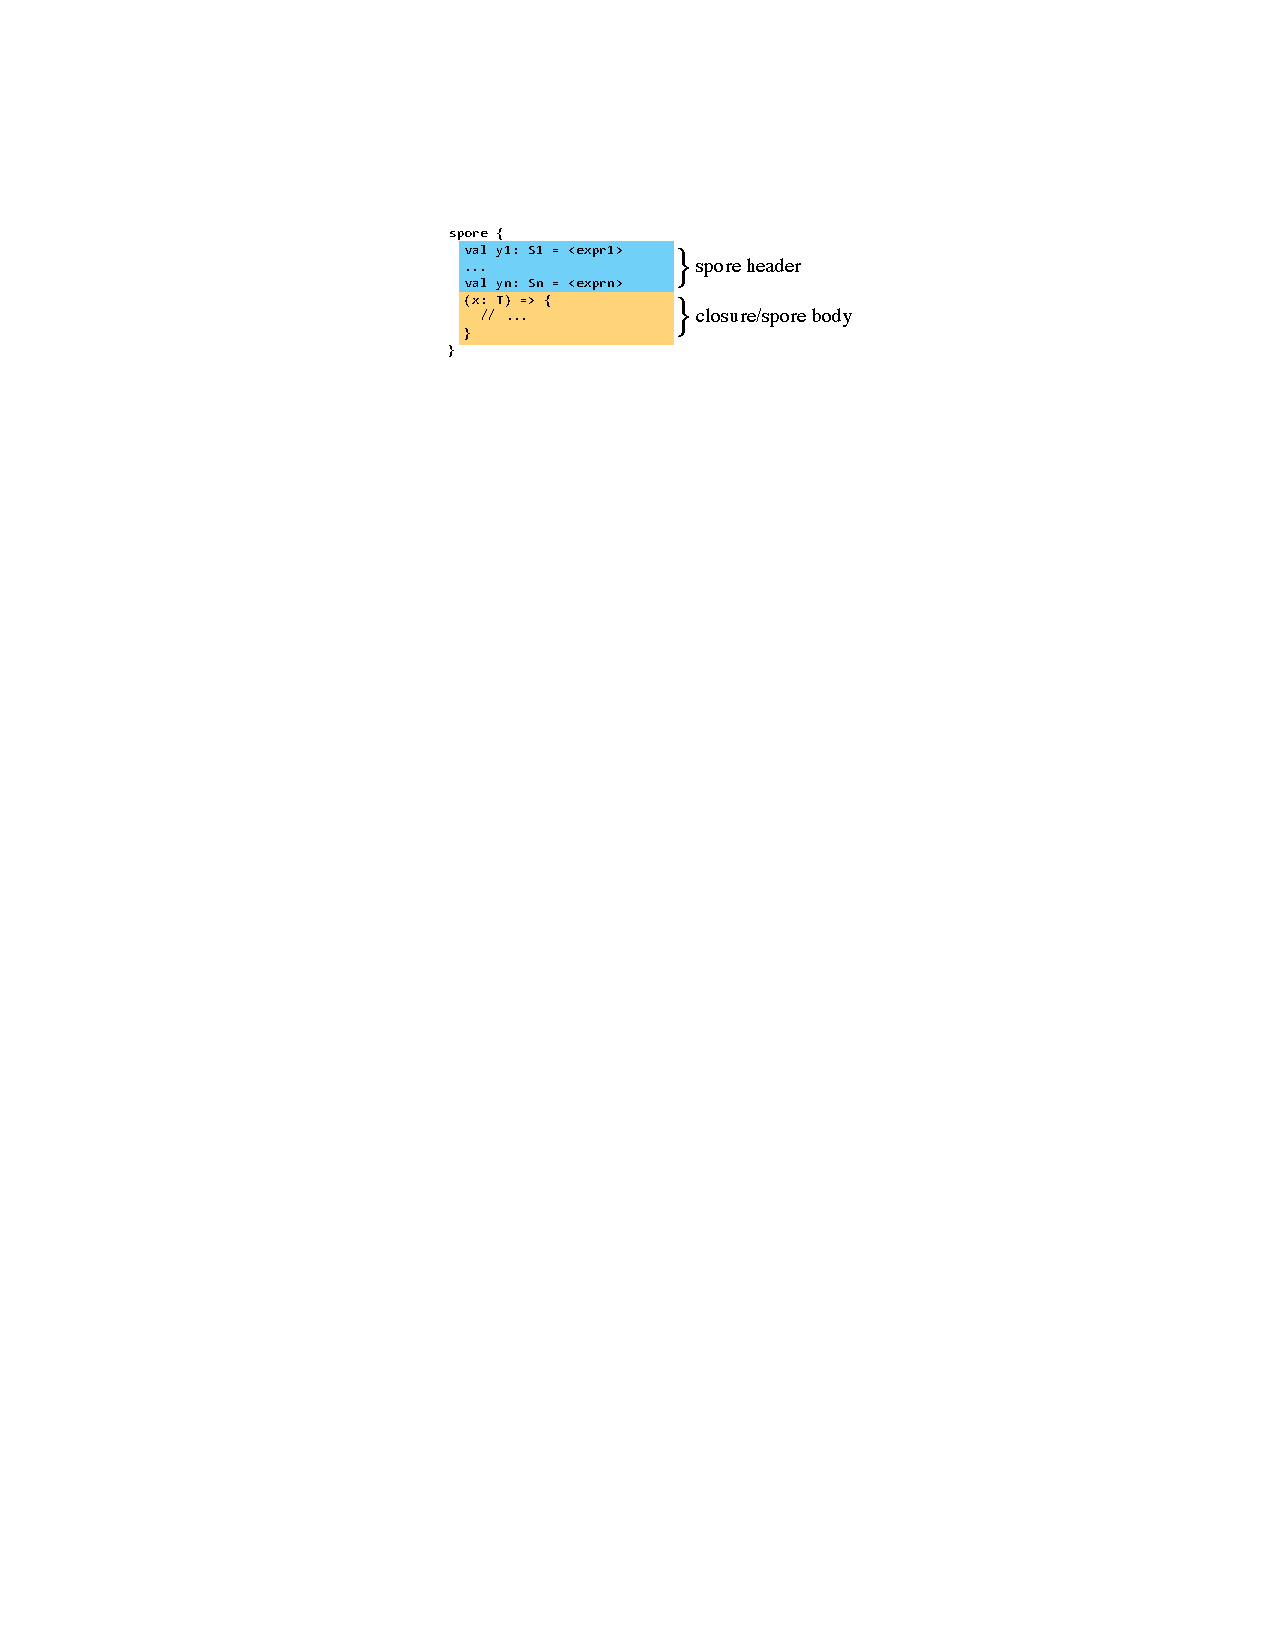
\includegraphics[width=0.75\columnwidth]{spore-shape.pdf}
\end{figure}
% \vspace{-1mm}

The characteristic property of a spore is that the spore body is only allowed
to access its parameter, the values in the spore header, as well as top-level
singleton objects (Scala's form of modules). The spore closure is not allowed
to capture variables other than those declared in the spore header (\ie a spore
may not capture variables in the environment). By enforcing this shape, the
environment of a spore is always declared explicitly in the spore header, which
avoids accidentally capturing problematic references. Moreover, importantly for
object-oriented languages like Scala, it's no longer possible to accidentally
capture the \verb|this| reference.

Spores also come with additional type-checking. Type information corresponding
to captured variables are included in the type of a spore. This enables authors
of distributed frameworks to customize type-checking of spores to, for example,
{\em exclude} a certain type from being captured by user-provided spores.
Authors of distributed frameworks opt into this type-checking by simply
including information about excluded types (or other type-based properties) in
the signature of a method. A concrete example would be to ensure that the
\verb|map| method on \verb|RDD|s in Spark (a distributed collection) accepts
only spores which do not capture \verb|SparkContext| (a non-serializable
internal framework class).

For a deeper understanding of spores, see
% either Appendix~\ref{appendix:spores} which covers the semantics of spores or
the corresponding publication~\cite{Spores}.

\begin{figure}[t!]
\centering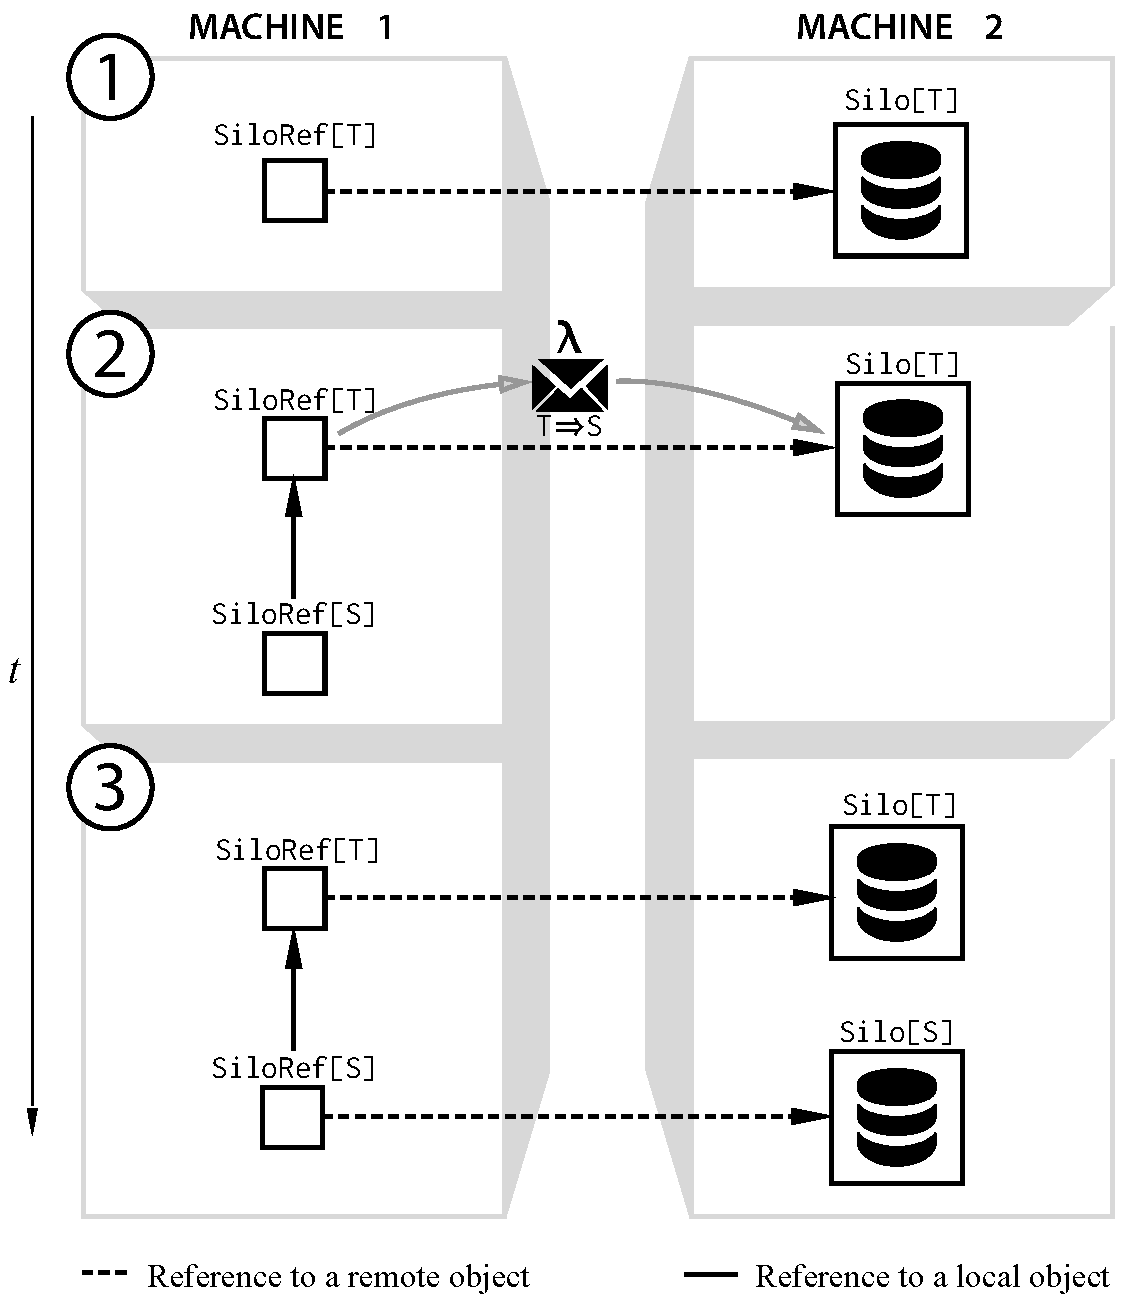
\includegraphics[width=0.8\columnwidth]{basic-diagram.pdf}
\caption{Basic function passing model.}\label{fig:basic-diagram}
\end{figure}

\subsection{Basic Usage}

We begin with a simple visual example to illustrate the basics of
the function passing model.
% \footnote{We also feel that, to visually illustrate a system
%   evolving in both space and time, nothing beats a video animation. So, we've
%   produced a short animation to provide visual intuition of the function passing model:
% \url{https://vimeo.com/120415626}}

The main handle users have to the framework is via SiloRefs. A SiloRef can be
thought of as an immutable handle to distributed data contained within a
corresponding silo. Users interact with this distributed data by applying
functions (as spores) to SiloRefs, which are transmitted over the wire and later
applied to the data within the corresponding silo. As is the case for persistent
data structures, when a function is applied to a piece of distributed data via a
SiloRef, a SiloRef representing a new silo containing the transformed data is
returned.

The simplest illustration of the model is shown in
Figure~\ref{fig:basic-diagram} (time flows vertically from top to bottom).
Here, we start with a \verb|SiloRef[T]| which points to a piece of remote data
contained within a \verb|Silo[T]|. When the function shown as $\lambda$ of type
$T \Rightarrow S$ is applied to \verb|SiloRef[T]| and ``forced'' (sent over the
wire), a new SiloRef of type \verb|SiloRef[S]| is immediately returned. Note
that \verb|SiloRef[S]| contains a reference to its parent SiloRef,
\verb|SiloRef[T]|. (This is how {\em lineages} are constructed.) Meanwhile, the
function is asynchronously sent over the wire and is applied to \verb|Silo[T]|,
eventually producing a new \verb|Silo[S]| containing the data transformed by
function $\lambda$. This new \verb|SiloRef[S]| can be used even before its
corresponding silo is materialized (\ie before the data in \verb|Silo[S]| is
computed) – the function passing framework queues up operations applied to \verb|SiloRef[S]|
and applies them when \verb|Silo[S]| is fully materialized.

Different sorts of complex DAGs can be asynchronously built up in this way.
Though first, to see how this is possible, we need to develop a clearer idea of
the primitive operations available on SiloRefs and their semantics. We describe
these in the following section.

\begin{figure}[t!]
\centering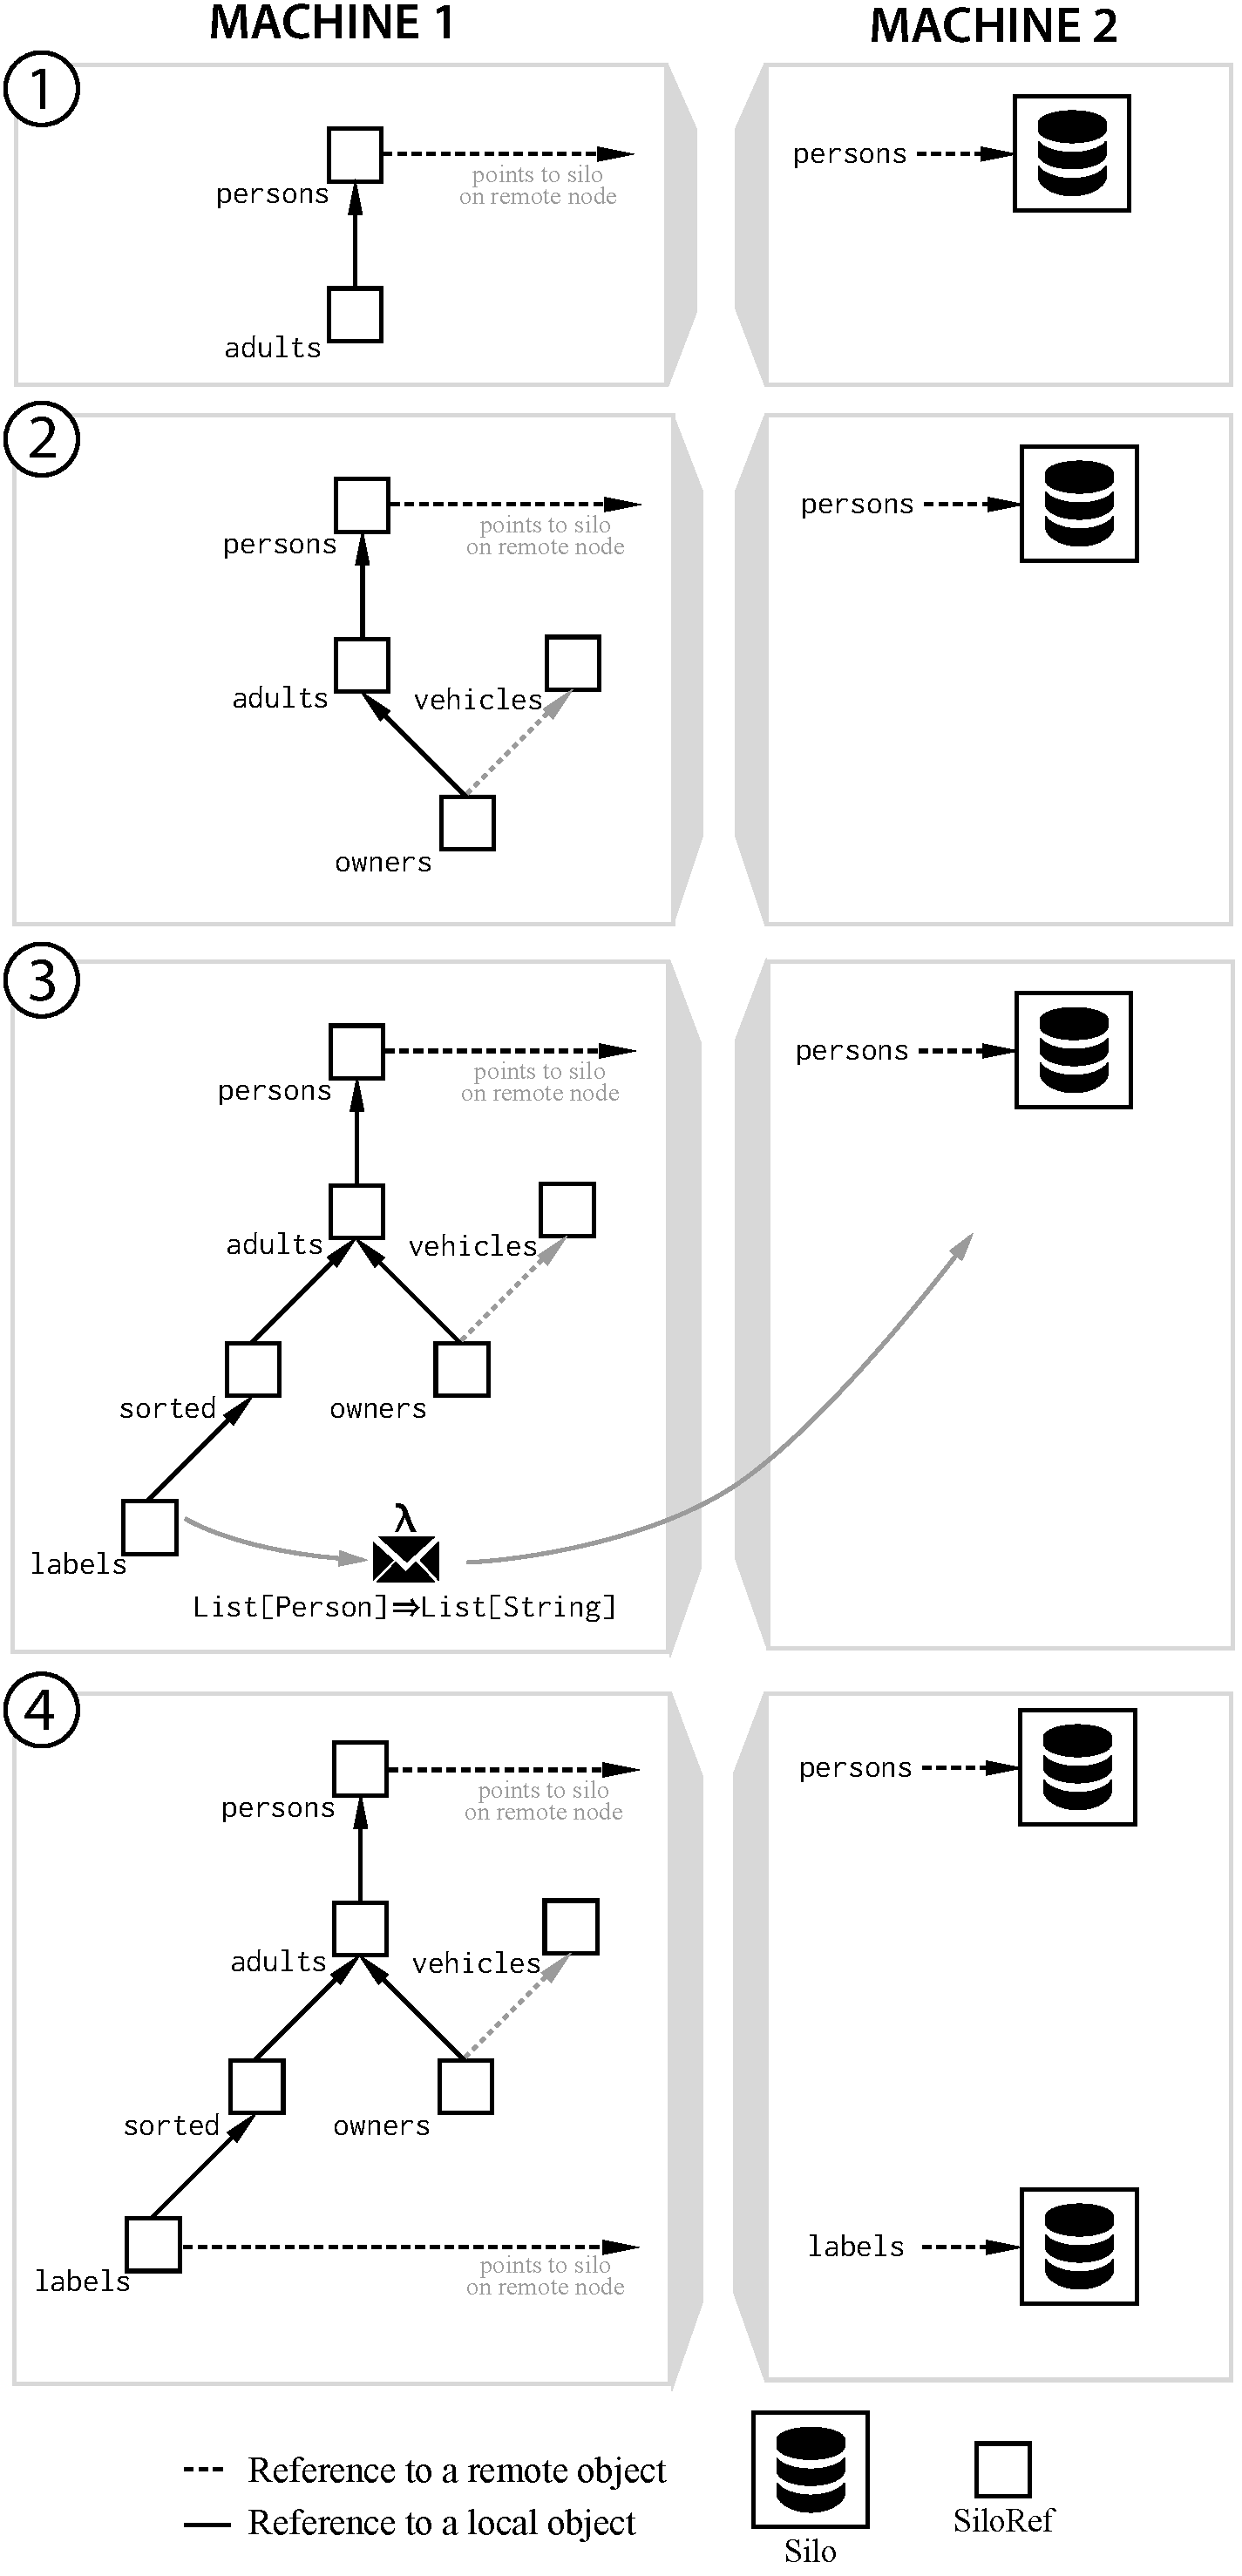
\includegraphics[width=\columnwidth]{bigger-dag.pdf}
\caption{A simple DAG in the function passing model.}\label{fig:bigger-dag}
\end{figure}

\subsection{Primitives}
\label{sec:primitives}

There are four basic primitive operations on SiloRefs that together can be used
to build the higher-order operations common to popular data-centric distributed
systems (how to build some of these higher-order operations is described in
Section~\ref{sec:higher-order-operations}). In this section we'll introduce
these primitives in the context of a running example. These primitives include:

\begin{itemize}[noitemsep,nolistsep]
\item \verb|map|
\item \verb|flatMap|
\item \verb|send|
\item \verb|cache|
\end{itemize}

\paragraph{map}%
%
\texttt{def map[S](s: Spore[T, S]): SiloRef[S]} \newline
%
The \verb|map| method takes a spore that is to be applied to the data in the
silo associated with the given SiloRef. Rather than immediately sending the
spore across the network, and waiting for the operation to finish, the
\verb|map| method's evaluation is \emph{deferred}. Without involving any network
communication, it immediately returns a SiloRef referring to a new,
soon-to-be-created silo. This new SiloRef only contains lineage information,
namely, a reference to the original SiloRef, a reference to the argument spore,
and the information that it is the result of a \verb|map| invocation. As we
explain below, another method, \verb|send| or \verb|cache|, must be called
explicitly to force the materialization of the result silo.

To better understand how DAGs are created and how remote silos are
materialized, we will develop a running example throughout this section. Given
a silo containing a list of \verb|Person| records, the following application of
\verb|map| defines a (not-yet-materialized) silo containing only the records of
adults (graphically shown in Figure~\ref{fig:bigger-dag}, part 1):

\begin{lstlisting}
val persons: SiloRef[List[Person]] = ...
val adults =
  persons.map(spore { ps => ps.filter(p => p.age >= 18) })
\end{lstlisting}

\paragraph{flatMap}%
%
\texttt{def flatMap[S](s: Spore[T, SiloRef[S]]): SiloRef[S]} \newline
%
Like \verb|map|, the \verb|flatMap| method takes a spore that is to be applied
to the data in the silo of the given SiloRef. However, the crucial difference
is in the type of the spore argument whose result type is a SiloRef in this
case. Semantically, the new silo created by \verb|flatMap| is defined to
contain the data of the silo that the user-defined spore returns.  The
\verb|flatMap| combinator adds expressiveness to our model that is essential to
express more interesting computation DAGs. For example, consider the problem of
combining the information contained in two different silos (potentially located
on different hosts). Suppose the information of a silo containing
\verb|Vehicle| records should be enriched with other details only found in the
\verb|adults| silo. In the following, \verb|flatMap| is used to create a silo
of \verb|(Person, Vehicle)| pairs where the names of person and vehicle owner
match (graphically shown in Figure~\ref{fig:bigger-dag}, part 2):

\begin{lstlisting}
val vehicles: SiloRef[List[Vehicle]] = ...
// adults that own a vehicle
val owners = adults.flatMap(spore {
  val localVehicles = vehicles // spore header
  ps =>
    localVehicles.map(spore {
      val localps = ps // spore header
      vs =>
        localps.flatMap(p =>
          // list of (p, v) for a single person p
          vs.flatMap {
            v => if (v.owner.name == p.name) List((p, v)) else Nil
          }
        )
    })
})
\end{lstlisting}
\noindent
Note that the spore passed to \verb|flatMap| declares the capturing of the
\verb|vehicles| SiloRef in its so-called ``spore header.'' The spore header
spans all variable definitions between the spore marker and the parameter list
of the spore's closure. The spore header defines the variables that the spore's
closure is allowed to access. Essentially, spores limit the free variables of
their closure's body to the closure's parameters and the variables declared in
the spore's header. Within the spore's closure, it is necessary to read the
data of the \verb|vehicles| silo in addition to the \verb|ps| list of
\verb|Person| records. This requires calling \verb|map| on
\verb|localVehicles|. However, \verb|map| returns a SiloRef; thus, invoking
\verb|map| on \verb|adults| instead of \verb|flatMap| would be impossible,
since there would be no way to get the data out of the silo returned by
\verb|localVehicles.map(..)|. With the use of \verb|flatMap|, however, the call
to \verb|localVehicles.map(..)| creates the final result silo, whose data is
then also contained in the silo returned by \verb|flatMap|.

Although the expressiveness of the \verb|flatMap| combinator subsumes that of
the \verb|map| combinator (see Section~\ref{sec:expr}), keeping \verb|map| as a
(lightweight) primitive enables more opportunities for optimizing computation
DAGs (\eg operation fusion~\cite{FlumeJava}).

\paragraph{send}%
%
\texttt{def send(): Future[T]} \newline
%
As mentioned earlier, the execution of computations built using SiloRefs is
deferred. The \verb|send| operation {\em forces} the deferred computation defined
by the given SiloRef.  Forcing is explicit in our model, because it requires
sending the lineage to the remote node on which the result silo should be
created. Given that network communication has a latency several orders of
magnitude greater than accessing a word in main memory, providing an explicit
send operation is a judicious choice~\cite{ANoteDistComp}.

To enable materialization of remote silos to proceed concurrently, the
\verb|send| operation immediately returns a future~\cite{Futures}. This future
is then asynchronously completed with the data of the given silo. Since calling
\verb|send| will materialize a silo and send its data to the current node,
\verb|send| should only be called on silos with reasonably small data (for
example, in the implementation of an aggregate operation such as \verb|reduce|
on a distributed collection).

\paragraph{cache}%
%
\texttt{def cache(): Future[Unit]} \newline
%
The performance of typical data analytics jobs can be increased dramatically by
caching large data sets in memory~\cite{Spark}. To do this, the silo containing
the computed data set needs to be materialized. So far, the only way to
materialize a silo that we have shown is using the \verb|send| primitive.
However, \verb|send| additionally transfers the contents of a silo to the
requesting node--too much if a large remote data set should merely be cached in
memory remotely.  Therefore, an additional primitive called \verb|cache| is
provided, which forces the materialization of the given SiloRef.

%, returning \verb|Future[Unit]|.

Given the running example so far, we can add another subgraph branching off of
\verb|adults|, which sorts each \verb|Person| by age, produces a \verb|String|
greeting, and then ``kicks-off'' remote computation by calling \verb|cache| and
caching the result in remote memory (graphically shown in
Figure~\ref{fig:bigger-dag}, part 3 and 4):

\begin{lstlisting}
val sorted =
  adults.map(spore { ps => ps.sortWith(p => p.age) })
val labels =
  sorted.map(spore { ps => ps.map(p => "Welcome, " + p.name) })
labels.cache()
\end{lstlisting}
\noindent
Assuming we would also cache the \verb|owners| SiloRef from the previous
example, the resulting lineage graph would look as illustrated in
Figure~\ref{fig:bigger-dag}. Note that \verb|vehicles|
is not a regular parent in the lineage of \verb|owners|; it is an indirect
input used to compute \verb|owners| by virtue of being {\em captured} by the
spore used to compute \verb|owners|.

% For example, Figure ?? shows the effect of invoking
% \verb|send| on the \verb|labels| SiloRef from above.

% The \verb|send| operation can also be used to simply cache a silo in main
% memory, for example, because the silo is known to be accessed subsequently:

% \paragraph{cache}
%
% The \verb|cache| method can be provided for convenience. It invokes
% \verb|send| not directly on the given SiloRef (which would transfer all data
% of the silo to the current node); instead, it first uses \verb|flatMap| to
% create a new silo that will be completed with the trivial value (e.g., a
% Boolean constant) of the \verb|DoneSiloRef| singleton object. Essentially,
% invoking \verb|send| on this trivial SiloRef causes the resulting future to
% be completed as soon as \verb|this| SiloRef has been materialized in main
% memory.

\subsubsection{Creating Silos}
\label{sec:creating-silos}

Besides a type definition for SiloRef, our framework provides a
companion singleton object (a Scala module). The singleton object
provides factory methods for obtaining SiloRefs referring to silos
populated with some initial data:\footnote{For clarity, only method
  signatures are shown.}

\begin{lstlisting}
object SiloRef {
  def fromTextFile(host: Host)(file: File):
                                      SiloRef[List[String]]
  def fromFun[T](host: Host)(s: Spore[Unit, T]): SiloRef[T]
  def fromLineage[T](host: Host)(s: SiloRef[T]): SiloRef[T]
}
\end{lstlisting}
\noindent
Each of the factory methods has a \verb|host| parameter that specifies the
target host (address/port) on which to create the silo. Note that the
\verb|fromFun| method takes a spore closure as an argument to make sure it can
be serialized and sent to \verb|host|. In each case, the returned SiloRef
contains its \verb|host| as well as a host-unique identifier. The
\verb|fromLineage| method is particularly interesting as it creates a copy of a
previously existing silo based on the lineage of a SiloRef \verb|s|. Note that
only the SiloRef is necessary for this operation to successfully complete; the
silo originally hosting \verb|s| might already have failed.

\subsubsection{Type Polymorphism and Silos/SiloRefs}

An important property of silos is that they are polymorphic in the type of data
that they hold. Importantly, silos are not just polymorphic in the {\em element
type} of their data, but in the {\em type of their entire dataset}. For example,
a silo might contain a Red-Black tree with elements of type \verb|Person| for
some ADT \verb|Person|, ordered by one of the fields of the \verb|Person| type.
Another silo might contain a completely different collection type, say, a linked
list. This type polymorphism enables optimizing silos according to their data
access patterns. Given that different data types may have specialized operations
(e.g., a tree map could provide a range projection), the key to enabling this
type polymorphism is the fact that a spore sent to a silo may apply arbitrary
functions to the silo's data. Thus, the SiloRef API itself is not limited to
providing just a fixed set of built-in operations (in contrast to RDDs in Spark,
for example).

\subsubsection{Expressiveness}
\label{sec:expr}

\paragraph{Expressing \texttt{map}}

Leveraging the above-mentioned methods for creating silos, it is possible to
express \verb|map| in terms of \verb|flatMap|:

\begin{lstlisting}
def map[S](s: Spore[T, S]): SiloRef[S] =
  this.flatMap(spore {
    val localSpore = s
    (x: T) =>
      val res = localSpore(x)
      SiloRef.fromFun(currentHost)(spore {
        val localRes = res
        () => localRes
      })
  })
\end{lstlisting}
\noindent
This should come as no surprise, given that \verb|flatMap| is the monadic bind
operation on SiloRefs, and \verb|SiloRef.fromFun| is the monadic return
operation. The reason why \verb|map| is provided as one of the main operations
of SiloRefs is that direct uses of \verb|map| enable an important optimization
based on operation fusion.

\paragraph{Expressing \texttt{cache}}

The \verb|cache| operation can be expressed using \verb|flatMap| and
\verb|send|:

\begin{lstlisting}
def cache(): Future[Unit] = this.flatMap(spore {
 val localDoneSiloRef = DoneSiloRef
 res => localDoneSiloRef
}).send()

\end{lstlisting}
\noindent
Here, we first use \verb|flatMap| to create a new silo that will be completed
with the trivial value of the \verb|DoneSiloRef| singleton object (\eg
\verb|Unit|). Essentially, invoking \verb|send| on this trivial SiloRef causes
the resulting future to be completed as soon as \verb|this| SiloRef has been
materialized in memory.


% This optimization is explained following the
% discussion of the third main operation of SiloRefs, \verb|send|.

% The type \verb|SiloRef[T]| has the following main operations:

% \begin{lstlisting}
% trait SiloRef[T] {
%   def map[S](s: Spore[T, S]): SiloRef[S]
%   def flatMap[S](s: Spore[T, SiloRef[S]]): SiloRef[S]
%   def send(): Future[T]
% }
% \end{lstlisting}

\subsection{Fault Handling}
\label{sec:fault-handling}

The function passing model includes overloaded variants of the primitives discussed so far which
enable the definition of flexible fault handling semantics. The main idea is to
specify fault handlers for \emph{subgraphs of computation DAGs}. Our guiding
principle is to make the definition of the failure-free path through a
computation DAG as simple as possible, while still enabling the handling of
faults at the fine-granular level of individual SiloRefs.

\paragraph{Defining Fault Handlers}

Fault handlers may be specified whenever the lineage of a SiloRef is extended.
For this purpose, the introduced \verb|map| and \verb|flatMap| primitives are
overloaded. For example, consider our previous example, but extended with a
fault handler:

\begin{lstlisting}
val persons: SiloRef[List[Person]] = ...
val vehicles: SiloRef[List[Vehicle]] = ...
// copy of `vehicles` on different host `h`
val vehicles2 = SiloRef.fromFun(h)(spore {
  val localVehicles = vehicles
  () => localVehicles
})

val adults =
  persons.map(spore { ps => ps.filter(p => p.age >= 18) })

// adults that own a vehicle
def computeOwners(v: SiloRef[List[Vehicle]]) =
  spore {
    val localVehicles = v
    (ps: List[Person]) => localVehicles.map(...)
  }

val owners: SiloRef[List[(Person, Vehicle)]] =
  adults.flatMap(computeOwners(vehicles),
                 computeOwners(vehicles2))
\end{lstlisting}

Importantly, in the \verb|flatMap| call on the last line, in addition to
\verb|computeOwners(vehicles)|, the regular spore argument of \verb|flatMap|,
\verb|computeOwners(vehicles2)| is passed as an additional argument. The second
argument registers a \emph{failure handler} for the subgraph of the computation
DAG starting at \verb|adults|. This means that if during the execution of
\verb|computeOwners(vehicles)| it is detected that the \verb|vehicles| SiloRef
has failed, it is checked whether the SiloRef that the higher-order combinator
was invoked on (in this case, \verb|adults|) has a failure handler registered.
In that case, the failure handler is used as an alternative spore to compute
the result of \verb|adults.flatMap(..)|. In this example, we specified
\verb|computeOwners(vehicles2)| as the failure handler; thus, in case
\verb|vehicles| has failed, the computation is retried using \verb|vehicles2|
instead.

\section{Higher-Order Operations}
\label{sec:higher-order-operations}

The introduced primitives enable expressing surprisingly intricate
computational patterns.

Higher-order operations such as variants of \verb|map|, \verb|reduce|, and
\verb|join|, operating on collections of data partitions, distributed across a
set of hosts, are required when implementing abstractions like Spark's
distributed collections~\cite{Spark}. Section~\ref{sec:dist-coll} demonstrates
the implementation of some such operations in terms of silos.

In addition, even more patterns are possible thanks to the decentralized nature
of our programming model, which removes the limitations of master/worker host
configurations. Section~\ref{sec:decentral} shows examples of peer-to-peer
patterns that are still fault-tolerant.

% \verb|union|, \verb|groupByKey|, or
% \verb|join|

\subsection{Higher-Order Operations}
\label{sec:dist-coll}

% \paragraph{union}
%
% The union of two unordered collections stored in two different silos can be
% expressed directly using the above \verb|flatMap| primitive.

\paragraph{join}

Suppose we are given two silos with the following types:

\begin{lstlisting}
val silo1: SiloRef[List[A]]
val silo2: SiloRef[List[B]]
\end{lstlisting}
\noindent
as well as two hash functions computing hashes (of type \verb|K|) for elements
of type \verb|A| and type \verb|B|, respectively:

\begin{lstlisting}
val hashA: A => K = ...
val hashB: B => K = ...
\end{lstlisting}
\noindent
The goal is to compute the hash-join of \verb|silo1| and \verb|silo2| using a
higher-order operation \verb|hashJoin|:

\begin{lstlisting}
def hashJoin[A, B, K](s1: SiloRef[List[A]],
                      s2: SiloRef[List[B]],
                      f: A => K,
                      g: B => K)
  : SiloRef[List[(K, (A, B))]] = ???
\end{lstlisting}
\noindent
To implement \verb|hashJoin| in terms of silos, the types of the two silos
first have to be made equal, through initial \verb|map| invocations:

\begin{lstlisting}
val s12: SiloRef[List[(K, Option[A], Option[B])]] =
  s1.map(spore { l1 => l1.map(x => (f(x), Some(x), None)) })
val s22: SiloRef[List[(K, Option[A], Option[B])]] =
  s2.map(spore { l2 => l2.map(x => (g(x), None, Some(x))) })
\end{lstlisting}
\noindent
Then, we can use \verb|flatMap| to create a new silo which contains the
elements of both silo \verb|s12| and silo \verb|s22|:

\begin{lstlisting}
val combined = s12.flatMap(spore {
  val localS22 = s22
  (triples1: List[(K, Option[A], Option[B])]) =>
    s22.map(spore {
      val localTriples1 = triples1
      (triples2: List[(K, Option[A], Option[B])]) =>
        localTriples1 ++ triples2
    })
})
\end{lstlisting}
\noindent
The combined silo contains triples of type \verb|(K, Option[A], Option[B])|.
Using an additional \verb|map|, the collection can be sorted by key, and
adjacent triples be combined, yielding a \texttt{SiloRef[List[(K, (A, B))]]} as
required.

\paragraph{Partitioning and groupByKey}

A \verb|groupByKey| operation on a group of silos containing collections needs
to create multiple result silos, on each node, with ranges of keys supposed to
be shipped to destination hosts. These destination hosts are determined using a
partitioning function. Our goal, concretely:

\begin{lstlisting}
val groupedSilos = groupByKey(silos)
\end{lstlisting}
\noindent
Furthermore, we assume that \verb|silos.size| $= N$ where $N$ is the number of
hosts, with hosts $h_1$, $h_2$, etc. We assume each silo contains an unordered
collection of key-value pairs (a multi-map). Then, \verb|groupByKey| can be
implemented as follows:

\begin{itemize}
\item Each host $h_i$ applies a {\em partitioning function} (example:
  \texttt{hash(key) mod N}) to the key-value pairs in its silo, yielding $N$
  (local) silos.

\item Using \verb|flatMap|, each pair of silos containing keys of the same
  range can be combined and materialized on the right destination host.
\end{itemize}

Using just the primitives introduced earlier, applying the partitioning
function in this way would require $N$ \verb|map| invocations per silo. Thus,
the performance of \verb|groupByKey| could be increased significantly using a
specialized combinator, say, ``mapPartition'' that would apply a given
partitioning function to each key-value pair, simultaneously populating $N$
silos (where $N$ is the number of ``buckets'' of the partitioning function).

\subsection{Peer-to-Peer Patterns}
\label{sec:decentral}

\subsubsection{Essence}

So far, our examples have focused on master-worker topologies that underly
models like Spark--\ie a master node specifies identical DAGs of computation for
all worker nodes to follow.

The function passing model, however, is not limited to these sorts of
topologies. It is indeed possible to develop decentralized, peer-to-peer
topologies on top of the function passing model. For example, a single compute
node may host silos that are remotely referenced by remote SiloRefs, as well as
SiloRefs remotely referencing silos on other compute nodes.

Further, as we show in the following example, it's also possible for multiple
clients to build completely different DAGs of computation off of some source
silo. In effect, this enables datasets to be shared--they exist once in memory
on some node, but can be used and transformed in different ways by different
clients.

Consider the following example. We start by populating an initial silo
representing a dataset of \verb|Vehicle| objects on
\verb|Host("lmpsrv1.scala-lang.org", 9999)|.

\begin{lstlisting}
val lmpsrv1 = Host("lmpsrv1.scala-lang.org", 9999)

// client #1
// populate initial silo
val vehicles: SiloRef[List[Vehicle]] =
  Silo.fromTextFile(lmpsrv1)("hdfs://...")

val silo2 = vehicles.map(spore {
  (vs: List[Vehicle]) =>
    // extract US state from license plate string, e.g, "FL329098"
    vs.map(v => (v.licensePlate.take(2), v)).toMap
})
val vehiclesPerState = silo2.send()

// client #2
// get siloref for silo that is being materialized due to client #1
val vehicles: SiloRef[List[Vehicle]] =
  Silo.fromTextFile(lmpsrv1)("hdfs://...")

val silo2 = vehicles.map(spore {
  // list all vehicles manufactured since 2013
  (vs: List[Vehicle]) => vs.filter(v => v.yearManufactured >= 2013)
})
val vehiclesSince2013 = silo2.send()
\end{lstlisting}

Here, client \#1 would like to perform some sort of computation based on the
states that vehicles are registered in. Another client, client \#2 would also
like to access this dataset. To do so, one must simply once again invoke
\verb|fromTextFile| on the same host, \verb|Host("lmpsrv1.scala-lang.org",9999)|
to obtain a SiloRef that points to a corresponding silo that is already or
soon to be materialized. From here, client \#2 is able to build an entirely
different DAG of computations, for instance in this example, filtering the
original \verb|vehicle| dataset to obtain only vehicles manufactured
since 2013.

\subsubsection{Decentralized Fault-Handling}

Another peer-to-peer pattern possible in the function passing model is
decentralized fault handling. One may specify strategies to transfer computation
to other nodes in the event of failure.

Consider the following example: an aggregation should be performed as
soon as two silos \verb|vehicles| and \verb|persons| have been
materialized. The aggregation result is then combined with a silo
\verb|info| on some host different from the local host. The final
result is written to a distributed file system:

\vspace{-0.8mm}
\begin{lstlisting}
object Utils {
  def aggregate(vs: SiloRef[List[Vehicle]],
                ps: SiloRef[List[Person]]): SiloRef[String] = ...
  def write(result: String, fileName: String): Unit = ...
}
val vehicles: SiloRef[List[Vehicle]] = ...
val persons:  SiloRef[List[Person]]  = ...
val info:     SiloRef[Info]          = ...
val fileName: String                 = "hdfs://..."
val done    = info.flatMap(spore {
  val localVehicles = vehicles
  val localPersons  = persons
  (localInfo: Info) =>
    aggregate(localVehicles, localPersons).map(spore {
      val in = localInfo
      res => combine(res, in)
    })
}).map(spore {
  val captured = fileName
  combined => Utils.write(combined, captured)
})
done.cache() // force computation
\end{lstlisting}
\noindent
This program does not tolerate failures of the host of \verb|info|: if
it fails before the computation is complete, the result is never
written to the file.

We can overcome this using fault handlers. It is possible to introduce
another backup host which takes over in case the host of \verb|info|
(which is the same as the host of \verb|done|) fails at any
point. Let's try the above computation again, this time using fault
handlers to transfer the computation to a backup node in the event of
a failure:

\begin{lstlisting}
val doCombine = spore {
  val localVehicles = vehicles
  val localPersons  = persons
  (localInfo: Info) =>
    aggregate(localVehicles, localPersons).map(spore {
      val in = localInfo
      res => combine(res, in)
    })
}
val doWrite = spore {
  val captured = fileName
  combined => Utils.write(combined, captured)
}
val done      = info.flatMap(doCombine).map(doWrite)
val backup    = SiloRef.fromFun(hostb)(spore { () => true })
val recovered = backup.flatMap(
  spore {
    val localDone = done
    x => localDone
  },
  spore { // fault handler
    val localInfo      = info
    val localDoCombine = doCombine
    val localDoWrite   = doWrite
    val localHostb     = hostb
    x =>
      // fromLineage makes sure, we re-run on hostb, rather than
      // the host of info. That is, we just duplicate the lineage.
      val restoredInfo = SiloRef.fromLineage(localHostb)(localInfo)
      restoredInfo.flatMap(localDoCombine).map(localDoWrite)
  }
)
done.cache()      // force computation on host of local
recovered.cache() // force computation on backup host
\end{lstlisting}
\noindent

First, the local variables \verb|doCombine| and \verb|doWrite| refer to the
verbatim spores passed to \verb|flatMap| and \verb|map| above. Second,
\verb|backup| is a dummy silo on a backup host \verb|hostb|. It is used to send
a spore to the backup host in a way that allows it to detect whether the
host of \verb|done|/\verb|info| has failed. The fault handling is done by calling \verb|flatMap|
on \verb|backup|, passing (a) a spore for the non-failure case and (b) a spore for
the failure case. The spore for the non-failure case simply returns the
\verb|done| SiloRef. Importantly, this enables \verb|hostb| to detect failures
of the host of \verb|done|. Upon detecting such a failure, \verb|backup.flatMap|
applies the spore for the failure case. In this case, the lineage of the
captured \verb|info| SiloRef is used to restore its original contents in a new
silo created on the backup host \verb|hostb|. Its SiloRef is then used to retry
the original computation.


% To illustrate the decentralized nature of our model, consider the following
% example: the local host aggregates some data as soon as two silos
% \verb|vehicles| and \verb|persons| have been materialized. The aggregation
% result is then combined with a silo \verb|info| on local host. The final result
% is written to a distributed file system:
%
% \begin{lstlisting}
% object Utils {
%   def aggregate(vs: SiloRef[List[Vehicle]],
%                 ps: SiloRef[List[Person]]): SiloRef[String] = ...
%   def write(result: String, fileName: String): Unit = ...
% }
% val vehicles: SiloRef[List[Vehicle]] = ...
% val persons:  SiloRef[List[Person]]  = ...
% val info:     SiloRef[Info]          = ...
% val fileName: String                 = "hdfs://..."
% val done    = info.flatMap(spore {
%   val localVehicles = vehicles
%   val localPersons  = persons
%   (localInfo: Info) =>
%     aggregate(localVehicles, localPersons).map(spore {
%       val in = localInfo
%       res => combine(res, in)
%     })
% }).map(spore {
%   val captured = fileName
%   combined => Utils.write(combined, captured)
% })
% done.cache() // force computation
% \end{lstlisting}
% \noindent
% This program does not tolerate failures of the local host: if it fails before
% the computation is complete, the result is never written to the file. Using
% fault handlers, though, it is easy to introduce a backup host that takes over
% in case the local host fails at any point:
%
% \begin{lstlisting}
% val doCombine = spore {
%   val localVehicles = vehicles
%   val localPersons  = persons
%   (localInfo: Info) =>
%     aggregate(localVehicles, localPersons).map(spore {
%       val in = localInfo
%       res => combine(res, in)
%     })
% }
% val doWrite = spore {
%   val captured = fileName
%   combined => Utils.write(combined, captured)
% }
% val done      = info.flatMap(doCombine).map(doWrite)
% val backup    = SiloRef.fromFun(hostb)(spore { () => true })
% val recovered = backup.flatMap(
%   spore {
%     val localDone = done
%     x => localDone
%   },
%   spore { // fault handler
%     val localInfo      = info
%     val localDoCombine = doCombine
%     val localDoWrite   = doWrite
%     val localHostb     = hostb
%     x =>
%       val restoredInfo = SiloRef.fromLineage(localHostb)(localInfo)
%       restoredInfo.flatMap(localDoCombine).map(localDoWrite)
%   }
% )
% done.cache()      // force computation on local host
% recovered.cache() // force computation on backup host
% \end{lstlisting}
% \noindent
% First, the local variables \verb|doCombine| and \verb|doWrite| refer to the
% verbatim spores passed to \verb|flatMap| and \verb|map| above. Second,
% \verb|backup| is a dummy silo on a backup host \verb|hostb|. It is used to send
% a spore to the backup host in a way that allows it to detect whether the
% original host has failed. The fault handling is done by calling \verb|flatMap|
% on \verb|backup|, passing (a) a spore for the non-failure case  (b) a spore for
% the failure case. The spore for the non-failure case simply returns the
% \verb|done| SiloRef. The spore for the failure case is applied whenever the
% value of the \verb|done| SiloRef could not be obtained. In this case, the
% lineage of the captured \verb|info| SiloRef is used to restore its original
% contents in a new silo created on the backup host \verb|hostb|. Its SiloRef is
% then used to retry the original computation. In case the original host failed
% only after the materialization of \verb|vehicles| and \verb|persons| completed,
% their cached data is reused.

% // concat
% def concat(silo1: SiloRef[List[A]],
%            silo2: SiloRef[List[A]]) =
%   silo1.flatMap(spore {
%     val localSilo2 = silo2
%     list1 =>
%       localSilo2.map(spore {
%         val localList1 = list1
%         list2 => localList1 ++ list2
%       })
%   })

% Operations on distributed collections\todo{somehow mention Spark here so it's
% clear what a dist coll is.}~such as \verb|union|, \verb|groupByKey|, or
% \verb|join|, involve multiple data sets, possibly located on different nodes.
% In the following we explain how such operations can be expressed using the
% introduced primitives.\todo{need a more compelling into for PL people}

\section{Formalization}
\label{sec:formalization}

While so far we have focused on a high-level description of our model,
visualizing, and building intuition via examples, we now shift gears
in an effort to make the primitives of our model more precise. Rather
than presenting a full formalization of our model, we will zoom in on
a few interesting highlights that fell out of our formalization. In
particular:
\begin{itemize}
  \item A new treatment of the concept of lineage using tools of the
    programming languages community as opposed to the way lineage has
    been studied in the database and systems communities.
  \item A newly-uncovered connection between type soundness and
    serializability.
\end{itemize}
\noindent
This is based on a formalization of our programming model in the
context of a typed lambda calculus with records. The full
formalization and the proof of a subject reduction theorem can be
found in the companion technical report~\cite{FPTechReport}.

\subsection{Formalizing Lineages}

In the following we formally model the concept of lineage which has
existed in other communities (in particular, the database and systems
communities), but which has not been treated in the context of
standard PL techniques such as small-step operational semantics.
Formalizing lineages is interesting for two reasons: first, our formal
model shows that lineages nicely map to and integrate with concepts
from functional programming. Second, the reduction relation of the
computation model is significantly different from standard reduction
relations for higher-order functional languages.

In the following we first summarize the abstract syntax of a core
language with essential constructs of our programming model. Then, we
provide an overview of reduction semantics, highlighting select
reduction rules for lineages.

\subsubsection{Syntax}

\begin{figure}[ht!]
\centering

$\ba[t]{l@{\hspace{2mm}}l}
t ::=                                                                  & \mbox{{\it{terms:}}} \\
\gap \:\:\:\:  x                                                       & \mbox{variable} \\
\gap ~|~  (x: T) \Rightarrow t                                         & \mbox{abstraction} \\
\gap ~|~  t~t                                                          & \mbox{application} \\
\gap ~|~  \{ \seq{l = t} \}                                            & \mbox{record} \\
\gap ~|~  t.l                                                          & \mbox{selection} \\
\gap ~|~  \texttt{spore}~\{~\seq{x : T = t}~; (x: T) \Rightarrow t~\}  & \mbox{spore} \\
\gap ~|~  \texttt{spawn}(t)                                            & \mbox{spawn host} \\
\gap ~|~  \texttt{populate}(t, t)                                      & \mbox{populate silo} \\
\gap ~|~  \texttt{map}(t, t)                                           & \mbox{map} \\
\gap ~|~  \texttt{flatMap}(t, t)                                       & \mbox{flatMap} \\
\gap ~|~  \texttt{persist}(t)                                          & \mbox{persist} \\
\gap ~|~  \texttt{send}(t)                                             & \mbox{send} \\           % send  :: Ref a -> Fut a
\gap ~|~  \texttt{await}(t)                                            & \mbox{await future} \\   % await :: Fut a -> a
\gap ~|~  \iota                                                        & \mbox{location} \\
\gap ~|~  r                                                            & \mbox{lineage} \\
                                                                       & \\
v ::=                                                                  & \mbox{{\it{values:}}} \\
\gap \:\:\:\: (x: T) \Rightarrow t                                     & \mbox{abstraction} \\
\gap ~|~  \{ \seq{l = v} \}                                            & \mbox{record value} \\
\gap ~|~  p                                                            & \mbox{spore value} \\
\gap ~|~  \iota                                                        & \mbox{location} \\
\gap ~|~  r                                                            & \mbox{lineage} \\
                                                                       & \\
p ::= \texttt{spore}~\{~\seq{x : T = v}~; (x: T) \Rightarrow t~\}      & \\
& \\
r ::=                                                  & \mbox{{\it{lineage:}}} \\
\gap \:\:\:\: \text{Mat}(\omega)                       & \mbox{materialized}             \\
\gap ~|~  \text{Mapped}(\omega, r, p)                  & \mbox{\texttt{map} lineage}     \\
\gap ~|~  \text{FMapped}(\omega, r, p)                 & \mbox{\texttt{flatMap} lineage} \\
\gap ~|~  \text{Persist}(\omega, r, v)                 & \mbox{\texttt{persist} lineage} \\
                                                       & \\
\omega  ::= (h,i) \quad \text{where}~i \in \mathbb{N}  & \mbox{identifier}      \\
& \\
T ::=                                                               & \mbox{{\it{types:}}} \\
\gap \:\:\:\: T \Rightarrow T                                       & \mbox{abstraction type} \\
\gap ~|~  \{ \seq{l : T} \}                                         & \mbox{record type} \\
\gap ~|~  T \Rightarrow T~\{~\texttt{type}~\mathcal{C} = \seq{T}~\} & \mbox{spore type} \\
\gap ~|~  \texttt{Host}                                             & \mbox{host type} \\
\gap ~|~  \texttt{SiloRef}[T]                                       & \mbox{lineage type} \\
\gap ~|~  \texttt{Future}[T]                                        & \mbox{future type}
\ea$
\caption{Abstract syntax of core language.}\label{fig:syntax}
\end{figure}

Figure~\ref{fig:syntax} shows the abstract syntax of our core
language. Besides standard terms, the language includes terms related
to (a) spores, (b) silos, and (c) futures. The \verb|spore| term
creates a new spore. It contains a list of variable definitions, the
spore header, and a closure which may only refer to its parameter and
variables in the spore header. The \verb|spawn| term creates a new
host capable of hosting silos. The \verb|populate| term initializes a
new silo on a given host with a given data value.  The \verb|map|,
\verb|flatMap|, and \verb|persist| terms create lineages of silo
transformations represented as silo references.  The \verb|send| term
forces the materialization of the silo corresponding to its argument
silo reference; \verb|send| returns a future which is asynchronously
completed with the silo's value. The \verb|await| term waits for the
completion of its argument future and returns the future's value.
Locations $\iota$ are used to refer to both futures and hosts.

Values in our language are as expected: besides abstractions and
record values they include spore values, locations, and
lineages. Locations and lineages are not part of the ``surface
syntax'' of our language; they are only introduced by reduction (see
Section~\ref{sec:reduction}). A lineage is a value of a simple
datatype with constructors {\em Mat, Mapped, FMapped}, and {\em
  Persist}. The constructors include all information required for {\em
  materializing} a silo with the result of applying the described
transformations. We defer a detailed explanation of the
transformations described by a lineage to the following
Section~\ref{sec:reduction}.

In addition to standard function and record types, the language has
types for spores, hosts, lineages, and futures. A spore type $T
\Rightarrow T'~\{~\texttt{type}~\mathcal{C} = \seq{T}~\}$ includes the
types $\seq{T}$ of the variables declared in the header of the
spore. (The name $\mathcal{C}$ stands for ``capture types''.)


\subsection{Reduction Semantics}\label{sec:reduction}

\begin{figure}
\centering
 $\ba[t]{l@{\hspace{2mm}}l}
E ::=                                                                                                     & \mbox{\it{eval. contexts:}} \\
\gap \:\:\:\: [~]                                                                                         & \mbox{hole} \\
\gap ~|~  E~t                                                                                             & \mbox{application (fun)} \\
\gap ~|~  v~E                                                                                             & \mbox{application (arg)} \\
\gap ~|~  \{ \seq{l = v} ; l_i = E ; \seq{l' = t} \}                                                      & \mbox{record} \\
\gap ~|~  E.l                                                                                             & \mbox{selection} \\
\gap ~|~  \texttt{spore}~\{~\seq{x : T = v} ; x_i : T_i = E ; & \\
\gap \gap                   \seq{x' : T = t} ; (x: T) \Rightarrow t~\}  & \mbox{spore} \\
\gap ~|~  \texttt{spawn}(E)                                                                               & \mbox{spawn} \\
\gap ~|~  \texttt{populate}(E, t)                                                                         & \mbox{populate (host)} \\
\gap ~|~  \texttt{populate}(v, E)                                                                         & \mbox{populate (spore)} \\
\gap ~|~  \texttt{map}(E, t)                                                                              & \mbox{map (ref)} \\
\gap ~|~  \texttt{map}(v, E)                                                                              & \mbox{map (fun)} \\
\gap ~|~  \texttt{flatMap}(E, t)                                                                          & \mbox{flatMap (ref)} \\
\gap ~|~  \texttt{flatMap}(v, E)                                                                          & \mbox{flatMap (fun)} \\
\gap ~|~  \texttt{persist}(E)                                                                             & \mbox{persist} \\
\gap ~|~  \texttt{send}(E)                                                                                & \mbox{send} \\
\gap ~|~  \texttt{await}(E)                                                                               & \mbox{await} \\
\ea$
\caption{Evaluation context.}\label{fig:eval-ctx}
\end{figure}

In the following we provide an overview of small-step operational
semantics of the introduced core language. The semantics are based on
three reduction relations for (a) sequential reduction of terms, (b)
deterministic reduction of hosts, and (c) non-deterministic reduction
of sets of hosts.  The reduction relations use the definition of
evaluation contexts shown in Figure~\ref{fig:eval-ctx}. Evaluation
contexts capture the notion of the ``next subterm to be evaluated.''
We write $E[t]$ for the term obtained by replacing the hole in
evaluation context $E$ with term $t$.


\paragraph{Notation and Conventions}

We write $S' = S + (\iota \mapsto v)$ to express the fact that $S'$ maps
$\iota$ to $v$ and otherwise agrees with $S$. We write $S(\iota) =
\text{Some}(v)$ to express the fact that $S$ maps $\iota$ to $v$. We write
$S(\iota) = \text{None}$ if $S$ does not have a mapping for $\iota$. Reduction
is defined using reduction contexts~\cite{TAPL}. We omit the definition of
reduction contexts, since they are completely standard.

\paragraph{Configurations}

The reduction rules of the deterministic layer define transitions of \emph{host
configurations} $(t, E, S)^h$ of host $h$ where $t$ is a term, $E$ is a message
queue, and $S$ is a silo store. The reduction rules of the non-deterministic
layer define transitions of sets $H$ of host configurations. The reduced host
configurations are chosen non-deterministically in order to express concurrency
between hosts.

\paragraph{Fault Handling}

In the interest of clarity we present the reduction rules in two steps. In the
first step we explain simplified rules without fault handling semantics
(Sections~\ref{sec:det-layer} and~\ref{sec:nondet-layer}). In the second step
we explain how these simplified rules have to be refined in order to support
the fault handling principles of our model (Section~\ref{sec:faults-opsem}).

\subsubsection{Decentralized Identification}

A important property of our programming model is the fact that silos are
uniquely identified using \emph{decentralized identifiers}. A decentralized
identifier $\iota$ has two components: (a) the identifier of the host $h$ that
created $\iota$, and (b) a name $i$ created fresh on $h$ (e.g., an integer
value): $\iota = (h, i)$. Decentralized identifiers are important, since they
reconcile two conflicting properties central to our model. The first property
is building computation DAGs locally, without remote communication. This is
possible using decentralized identifiers, since each host can generate new
identifiers independently of other remote hosts. The second property is
allowing SiloRefs to be freely copied between remote hosts. This is possible,
since decentralized identifiers uniquely identify silos without the need for
subsequent updates of their information; decentralized identifiers are
immutable. This latter property is essential to enable computation DAGs that
are \emph{immutable upon construction}. In our programming model, computation
DAGs are created using the standard monadic operations of SiloRefs. In
particular, the \texttt{flatMap} operation (monadic bind) in general requires
that its argument spore captures SiloRefs that are subsequently copied to a
remote host. Hence it is essential that SiloRefs and the decentralized
identifiers they contain be freely copyable between remote hosts.

\begin{figure*}[t!]
  \centering
% \vspace{-7mm}
\begin{mathpar}

\inferrule[\textsc{R-Send}]
{ host(r) = h' \quad h' \neq h \quad i~\text{fresh} \\
  \iota = (h, i) \quad m = \text{Req}(h, r, \iota)
}
{ \{ (R[\texttt{send}(r)], E, S)^h, (t, E', S')^{h'} \} \cup H \rightarrow \{ (R[\iota], E, S)^h, (t, E' \cdot m, S')^{h'} \} \cup H
}

\inferrule[\textsc{R-Req1}]
{ E = \text{Req}(h', r, \iota') \texttt{::} E' \quad r = \text{Mat}(\iota) \\
  S(\iota) = \text{Some}(v) \quad m = \text{Res}(\iota', v)
}
{ \{ (R[\texttt{await}(\iota_f)], E, S)^h, (t, E'', S')^{h'} \} \cup H \rightarrow \{ (R[\texttt{await}(\iota_f)], E', S)^h, (t, E'' \cdot m, S')^{h'} \} \cup H
}

\inferrule[\textsc{R-Req2}]
{ E = \text{Req}(h', r, \iota') \texttt{::} E' \quad r = \text{Mapped}(\iota, h, r', p, \text{None}) \quad r' = \text{Mat}(\iota_s) \quad S(\iota) = \text{None} \\
  S(\iota_s) = \text{Some}(v) \quad p(v) = v' \quad S' = S + (\iota \mapsto v') \quad m = \text{Res}(\iota', v')
}
{ \{ (R[\texttt{await}(\iota_f)], E, S)^h, (t, E'', S'')^{h'} \} \cup H \rightarrow \{ (R[\texttt{await}(\iota_f)], E', S')^h, (t, E'' \cdot m, S'')^{h'} \} \cup H
}

\inferrule[\textsc{R-Req3}]
{ E = \text{Req}(h'', r, \iota'') \texttt{::} E'' \quad r = \text{FMapped}(\iota, h, \text{Mat}(\iota_s), p, \text{None}) \quad S(\iota) = \text{None} \quad S(\iota_s) = \text{Some}(v) \\
  \quad p(v) = r' \quad loc(r') = \iota' \quad S(\iota') = \text{None} \quad host(r') = h' \quad m = \text{Req}(h, r', \iota') \quad E''' = \text{Req}(h'', r', \iota'') \texttt{::} E''
}
{ \{ (R[\texttt{await}(\iota_f)], E, S)^h, (t, E', S')^{h'} \} \cup H \rightarrow \{ (R[\texttt{await}(\iota_f)], E''', S)^h, (t, E' \cdot m, S')^{h'} \} \cup H
}

\inferrule[\textsc{R-Req4}]
{ E = \text{Req}(h'', r, \iota'') \texttt{::} E'' \quad r = \text{FMapped}(\iota, h, \text{Mat}(\iota_s), p, \text{None}) \quad S(\iota) = \text{None} \quad S(\iota_s) = \text{Some}(v) \\
  \quad p(v) = r' \quad loc(r') = \iota' \quad S(\iota') = \text{Some}(v') \quad S'' = S + (\iota \mapsto v') \quad m = \text{Res}(\iota'', v')
}
{ \{ (R[\texttt{await}(\iota_f)], E, S)^h, (t, E', S')^{h''} \} \cup H \rightarrow \{ (R[\texttt{await}(\iota_f)], E'', S'')^h, (t, E' \cdot m, S')^{h''} \} \cup H
}

\end{mathpar}
  % \vspace{-3mm}
  \caption{Nondeterministic reduction.}
  \label{fig:opsem-nondeterm}
  % \vspace{-3mm}
\end{figure*}

\subsubsection{Deterministic Layer}
\label{sec:det-layer}

We first consider the reduction rules of the deterministic layer shown in
Figure~\ref{fig:opsem-determ}. The reduction rules for \texttt{map}
(\textsc{R-Map}) and \texttt{flatMap} (\textsc{R-FMap}) do not involve
communication with other hosts. In each case, a new SiloRef $r'$ is created
that is derived from SiloRef $r$. The execution of the actual operation
(\texttt{map} or \texttt{flatMap}, respectively) is deferred, and an object
representing this derivation is returned. In both cases, the new SiloRef $r'$
refers to a silo created on host $h'$ by applying the spore value $p$ to the
value of silo $r$. The first component of the Mapped and FMapped objects, $(h,
i)$, is a fresh \emph{location} created by host $h$ to uniquely identify the
result silo.

Most reduction rules are enabled when the current redex is an \texttt{await}
term. The reduction of a term $\texttt{await}(\iota)$ only continues when store
$S$ maps location $\iota$ to value $v$. In all other cases, the current host
removes the next message from its message queue $E$. As shown in
Figure~\ref{fig:elems-opsem} there are two types of messages: requests (Req)
and responses (Res). A response $\text{Res}(\iota, v)$ tells its receiver that
the silo at location $\iota$ has value $v$. A request $\text{Req}(h, r, \iota)$
is sent on behalf of host $h$ to request the value of silo $r$ at location
$\iota$. The reception of a response $\text{Res}(\iota, v)$ is handled by
adding a mapping $(\iota \mapsto v)$ to the store (rule \textsc{R-Res}). The
reception of a request $\text{Req}(h', r, \iota'')$ is handled locally if
materialization of the requested silo $r$ is deferred and the parent silo $r'$
in $r$'s lineage has not been materialized either. In this case, the host sends
a request to materialize $r'$ to itself.



\subsubsection{Nondeterministic Layer}
\label{sec:nondet-layer}

All reduction rules in the nondeterministic layer, shown in
Figure~\ref{fig:opsem-nondeterm}, involve communication between two hosts.

Reducing a term $\texttt{send}(r)$ appends a request $\text{Req}(h, r, \iota)$
to the message queue of host $h'$ of the requested silo $r$. In this case, host
$h$ creates a unique location $\iota = (h, i)$ to identify the silo
subsequently. Rules \textsc{R-Req1}, \textsc{R-Req2}, and \textsc{R-Req3}
define the handling of request messages that cannot be handled locally. If the
request can be serviced immediately (\textsc{R-Req1}), a response with the
value $v$ of the requested silo $r$ is appended to the message queue of the
requesting host $h'$. Rules \textsc{R-Req2} and \textsc{R-Reg3} handle cases
where the requested silo is not already available in materialized form.

% Failures may be detected whenever a message is sent to a non-local host. Note that this does not mean that message sends must be synchronous. Instead, our implementation interprets a failure to establish a network connection with a remote host as a failure of the remote host and thus a failure of all silos that it hosts.

\begin{figure*}[t!]
  \centering
% \vspace{-7mm}
\begin{mathpar}

\inferrule[\textsc{RF-Send}]
{ host(r) = h' \quad h' \neq h \quad \text{failed}(h') \\
  \quad i~\text{fresh} \quad \iota = (h, i) \quad S'' = S + (\iota \mapsto \bot)
}
{ \{ (R[\texttt{send}(r)], E, S)^h \} \cup H \rightarrow \{ (R[\iota], E, S'')^h \} \cup H
}

\inferrule[\textsc{RF-Req4}]
{ E = \text{Req}(h'', r, \iota'') \texttt{::} E'' \quad r = \text{FMapped}(\iota, h, r'', p, \text{Some}(p_f)) \quad S(\iota) = \text{None} \\
  loc(r'') = \iota_s \quad S(\iota_s) = \text{Some}(v) \quad p(v) = r' \quad \text{failed}(host(r')) \quad p_f(v) = r_f \quad host(r_f) = h_f \quad \lnot \text{failed}(h_f) \\
  loc(r_f) = \iota_f \quad S(\iota_f) = \text{None} \quad m = \text{Req}(h, r_f, \iota_f) \quad E''' = \text{Req}(h'', r_f, \iota'') \texttt{::} E''
}
{ \{ (R[\texttt{await}(\iota_f)], E, S)^h, (t, E', S')^{h_f} \} \cup H \rightarrow \{ (R[\texttt{await}(\iota_f)], E''', S)^h, (t, E' \cdot m, S')^{h_f} \} \cup H
}

\inferrule[\textsc{RF-Req5}]
{ E = \text{Req}(h'', r, \iota'') \texttt{::} E' \quad r = \text{FMapped}(\iota, h, r'', p, \text{None}) \quad S(\iota) = \text{None} \quad loc(r'') = \iota_s \quad S(\iota_s) = \text{Some}(v) \\
  p(v) = r' \quad \text{failed}(host(r')) \quad i_p, i_a~\text{fresh} \quad \iota_p = (h, i_p), \iota_a = (h, i_a) \quad m_p = \text{ReqF}(h, r'', \iota_p) \\
  r_a = \text{FMapped}(\iota_a, h, \text{Mat}(\iota_p), p, \text{None}) \quad E'' = m_p \texttt{::} \text{Req}(h'', r_a, \iota'') \texttt{::} E'
}
{ (R[\texttt{await}(\iota_f)], E, S)^h \longrightarrow (R[\texttt{await}(\iota_f)], E'', S)^h
}

\inferrule[\textsc{RF-ReqF}]
{ E = \text{ReqF}(h, r, \iota') \texttt{::} E' \quad r = \text{Mapped}(\iota, h, r'', p, \text{Some}(p_f)) \\
  loc(r'') = \iota_s \quad S(\iota_s) = \text{Some}(v) \quad E'' = \text{Res}(\iota', p_f(v)) \texttt{::} E'
}
{ (R[\texttt{await}(\iota_f)], E, S)^h \longrightarrow (R[\texttt{await}(\iota_f)], E'', S)^h
}

\end{mathpar}
  \vspace{-3mm}
  \caption{Fault handling.}
  \label{fig:opsem-faults}
  \vspace{-3mm}
\end{figure*}

% \vspace{-2.25mm}
\subsection{Fault Handling}
\label{sec:faults-opsem}
% \vspace{-1mm}
The key principles of the fault handling mechanism are:
% \vspace{-1mm}
\begin{itemize}
\item Whenever a message is sent to a non-local host $h$, it is checked whether
  $h$ is alive; if it is not, any silos located on $h$ are declared to have
  failed.
\item Whenever the value of a silo $r$ cannot be obtained due to another failed
  silo, $r$ is declared to have failed.
\item Whenever the failure of a silo $r$ is detected, the nearest predecessor
  $r'$ in $r$'s lineage that is not located on the same host is determined. If
  $r'$ has a fault handler $f$ registered, the execution of $f$ is requested.
  Otherwise, $r'$ is declared to have failed.
\end{itemize}

% A host either (a) discovers itself that a remote silo has failed (e.g., because it could not establish a network connection to the remote host), or (b) is notified that a remote silo has failed by a healthy host involved in its materialization.

These principles are embodied in the reduction as follows. First, we use the
predicate $\text{failed}(h)$ as a way to check whether it is possible to
communicate with host $h$ (e.g., an implementation could check whether it is
possible to establish a socket connection). Second, failures of hosts are
handled whenever communication is attempted: whenever a host $h$ intends to
send a message to a host $h'$ where $h' \neq h$, it is checked whether
$\text{failed}(h')$. If it is the case that $\text{failed}(h')$, either the
corresponding location (silo or future) is declared as failed (and fault
handling deferred), or a suitable fault handler is located and a recovery step
is attempted. In the following we explain the extended reduction rules shown in
Figure~\ref{fig:opsem-faults}.

In rule \textsc{RF-Send}, the host of the requested silo $r$ is detected to
have failed. However, the parent silos of $r$ are all located on the same
(failed) host. Thus, in this case silo $r$ is simply declared as failed, and
fault handling is delegated to other parts of the computation DAG that require
the value of $r$ (if any). Since \texttt{send} is essentially a ``sink'' of a
DAG, no suitable fault handler can be located at this point.

This is different in rule \textsc{RF-Req4}. Here, host $h$ processes a message
requesting silo $r$ which is the result of a \texttt{flatMap} call.
Materializing $r$ requires obtaining the value of silo $r'$, the result of
applying spore $p$ to the value $v$ of the materialized parent $r''$.
Importantly, if the host of $r'$ is failed, it means the computation of the DAG
defined by spore $p$ did not result in a silo on an available host.
Consequently, if the \texttt{flatMap} call deriving $r$ specified a fault
handler $p_f$, $p_f$ is applied to $v$ in order to recover from the failure.
If the host of the resulting silo $r_f$ is not failed, the original request for
$r$ is ``modified'' to request $r_f$ instead. This is done by removing message
$\text{Req}(h'', r, \iota'')$ from the message queue and prepending message
$\text{Req}(h'', r_f, \iota'')$. Moreover, host $h$ sends a message to itself,
requesting the value of silo $r_f$.

Rule \textsc{RF-Req5} shows fault recovery in the case where the lineage of a
requested silo does not specify a fault handler itself. In this case, host $h$
creates two fresh locations $\iota_p, \iota_a$. $\iota_p$ is supposed to be
eventually mapped to the result value of executing the fault handler of parent
silo $r''$. Host $h$ requests this value from itself using a special message
$\text{ReqF}(h, r'', \iota_p)$. Finally, the original request for silo $r$ in
message queue $E$ is replaced with a request for silo $r_a$. The silo $r_a$ is
created analogous to $r$, but using silo $\text{Mat}(\iota_p)$ as parent
(eventually, location $\iota_p$ is mapped to the result of applying the
parent's fault handler). As demonstrated by rule \textsc{RF-ReqF}, ReqF
messages used to request the application of the fault handler are handled in a
way that is completely analogous to the way regular Req messages are handled,
except that fault handlers $p_f$ are applied as opposed to regular spores $p$.

\section{Implementation}
\label{sec:implementation}

The presented programming model has been fully implemented in Scala, a
functional programming language that runs on both JVMs and JavaScript runtimes.
The function passing model is compiled and run using Scala 2.11.8, and considers only the JVM backend
for now. Our implementation, which has been published as an open-source
project,\footnote{\url{https://github.com/heathermiller/f-p}} builds on two
main Scala extensions:

\begin{itemize}

\item First, Pickling~\cite{Pickling},\footnote{\url{https://github.com/scala/pickling}}
  a type-safe and performant serialization library with an accompanying, optional
  macro extension that is focused on distributed programming. It is used for
  all serialization tasks. Our function passing implementation benefits from the maturity of
  Pickling, which supports pickling/unpickling a wide range of Scala type
  constructors. Pickling has evolved from a research prototype to a
  production-ready serialization framework that is now in widespread commercial
  use.

\item Second, the programming model makes extensive use of spores, closure-like
  objects with explicit, typed environments. While~\cite{Spores} has reported an
  an empirical evaluation of spores, our presented programming model and
  implementation turned out to be an extensive validation of spores in the context
  of distributed programming. In addition, our implementation required a thorough
  refinement of the way spores are pickled.

\end{itemize}

So far, we have used our implementation to build a small Spark-like distributed
collections abstraction, a simple version of the MBrace~\cite{MBrace} framework,
and example data analytics applications, such as word count and group-by-join
pipelines. We give an introduction and step through some of these example
applications in section~\ref{sec:examples}.

% Our prototype has also served as an experimentation platform for
% type-based optimizations, which we present in more detail below.

% Further, we maintain a growing collection of these toy distributed frameworks
% (built on top of function passing) and applications on top of them (such as data analytics)
% at \url{http://lampwww.epfl.ch/~hmiller/f-p/}.\footnote{Review note: this site
%   is publicly accessible, has no tracking capabilities, and is linked to in
% talks and from other various webpages meaning it already gets public traffic.
% One may visit it without identity concerns.}

\subsection{Static Serialization and Generics}

In a function passing program, code using \verb|SiloRef|s may access multiple
silos hosted on different remote nodes. Therefore, applying a combinator such as
\verb|map| to a \verb|SiloRef| generally requires sending a message to a remote
node instructing it to apply \verb|map| to the contents of the corresponding
silo. For example, consider the following invocation of \verb|map| on a SiloRef
\verb|in|:

\begin{lstlisting}
val out =
  in.map(spore { (l: List[String]) => l.map(_.toUpperCase) })
\end{lstlisting}

The above snippet takes a list of strings in an input silo \verb|in| and
produces an output silo \verb|out| containing the list with each string in upper
case.

Assuming that the silo that \verb|in| refers to is hosted on some remote node
$RN$, materializing \verb|out| (on the same node) requires sending a message
representing this \verb|map| invocation to $RN$. In the above example, the
materialization of \verb|out| would entail sending an instance of a class
\verb|Mapped[T, S]| where \verb|T = S = List[String]| to $RN$.

While serializing the instance of \verb|Mapped| with the concrete type
\verb|Mapped[List[String], List[String]]| is straightforward, the key question
is: how to deserialize this on $RN$?

Importantly, the combinator code on the server-side is generic; it is not
specific to any client code where types are made concrete.

In the example, this means that the concrete type argument \verb|List[String]|
is only known at run time on $RN$. As a result, the remote node must interpret
the run-time type on the fly in order to deserialize the instance of
\verb|Mapped|.

Such interpretation-based deserializers are know to be significantly slower than
type-specific, statically-generated deserializers~\cite{Pickling}. In fact, a
recent study has identified serialization as a major bottleneck in
data-intensive applications~\cite{Ousterhout}, one of our main target
applications.

In order to minimize the cost of deserialization, we have devised a
serialization scheme that enables utilizing statically-generated deserializers,
thereby avoiding the performance penalty of interpretation-based deserializers.

The approach which we call ``self-describing pickles'' is as follows. Basically,
the idea is to augment the serialized representation with additional information
about how to deserialize (``unpickle'') it. The key is to capture the
type-specific pickler and unpickler when the fully-concrete type of a
\verb|Mapped| instance is known:

\begin{lstlisting}
def doPickle[T](msg: T)
  (implicit pickler: Pickler[T],
               unpickler: Unpickler[T]): Array[Byte] = ...
\end{lstlisting}

Essentially, this means when \verb|doPickle| is called with a concrete type \verb|T|, say:\footnote{Note that the type arguments are inferred by the Scala compiler; they are only shown for clarity.}

\begin{lstlisting}
doPickle[Mapped[List[Int], List[String]]](mapped)
\end{lstlisting}

\noindent not only a type-specific implicit pickler (a type class instance) is
looked up, but also a type-specific implicit *unpickler*. The \verb|doPickle|
method can then build a self-describing pickle as follows. First, the actual
message is pickled using the pickler, yielding a byte array. Then, an instance
of the following simple record-like class is created:

\begin{lstlisting}
case class SelfDescribing(blob: Array[Byte],
                          unpicklerClassName: String)
\end{lstlisting}

Besides the just produced byte array, it contains the class name of the
type-specific unpickler. This enables using this fully type-specific unpickler,
even when the message type to be unpickled is only partially known. All that is
required is an unpickler for type \verb|SelfDescribing|. First, it reads the
byte array and class name from the pickle. Second, it instantiates the
type-specific unpickler reflectively using the class name. (Note that this is
possible on both the JVM as well as on JavaScript runtimes using Scala's current
JavaScript backend.) Finally, the unpickler is used to unpickle the byte array.
In conclusion, this approach ensures (a) that a type that is pickleable using a
type-specific pickler is guaranteed to be unpickleable by the receiver of the
pickled \verb|SelfDescribing| instance, and (b) that unpickling is as efficient
as pickling, thanks to using type-specific unpicklers.

% \subsection{Type-based optimization of serialization}

% \begin{figure}[t!]
% \centering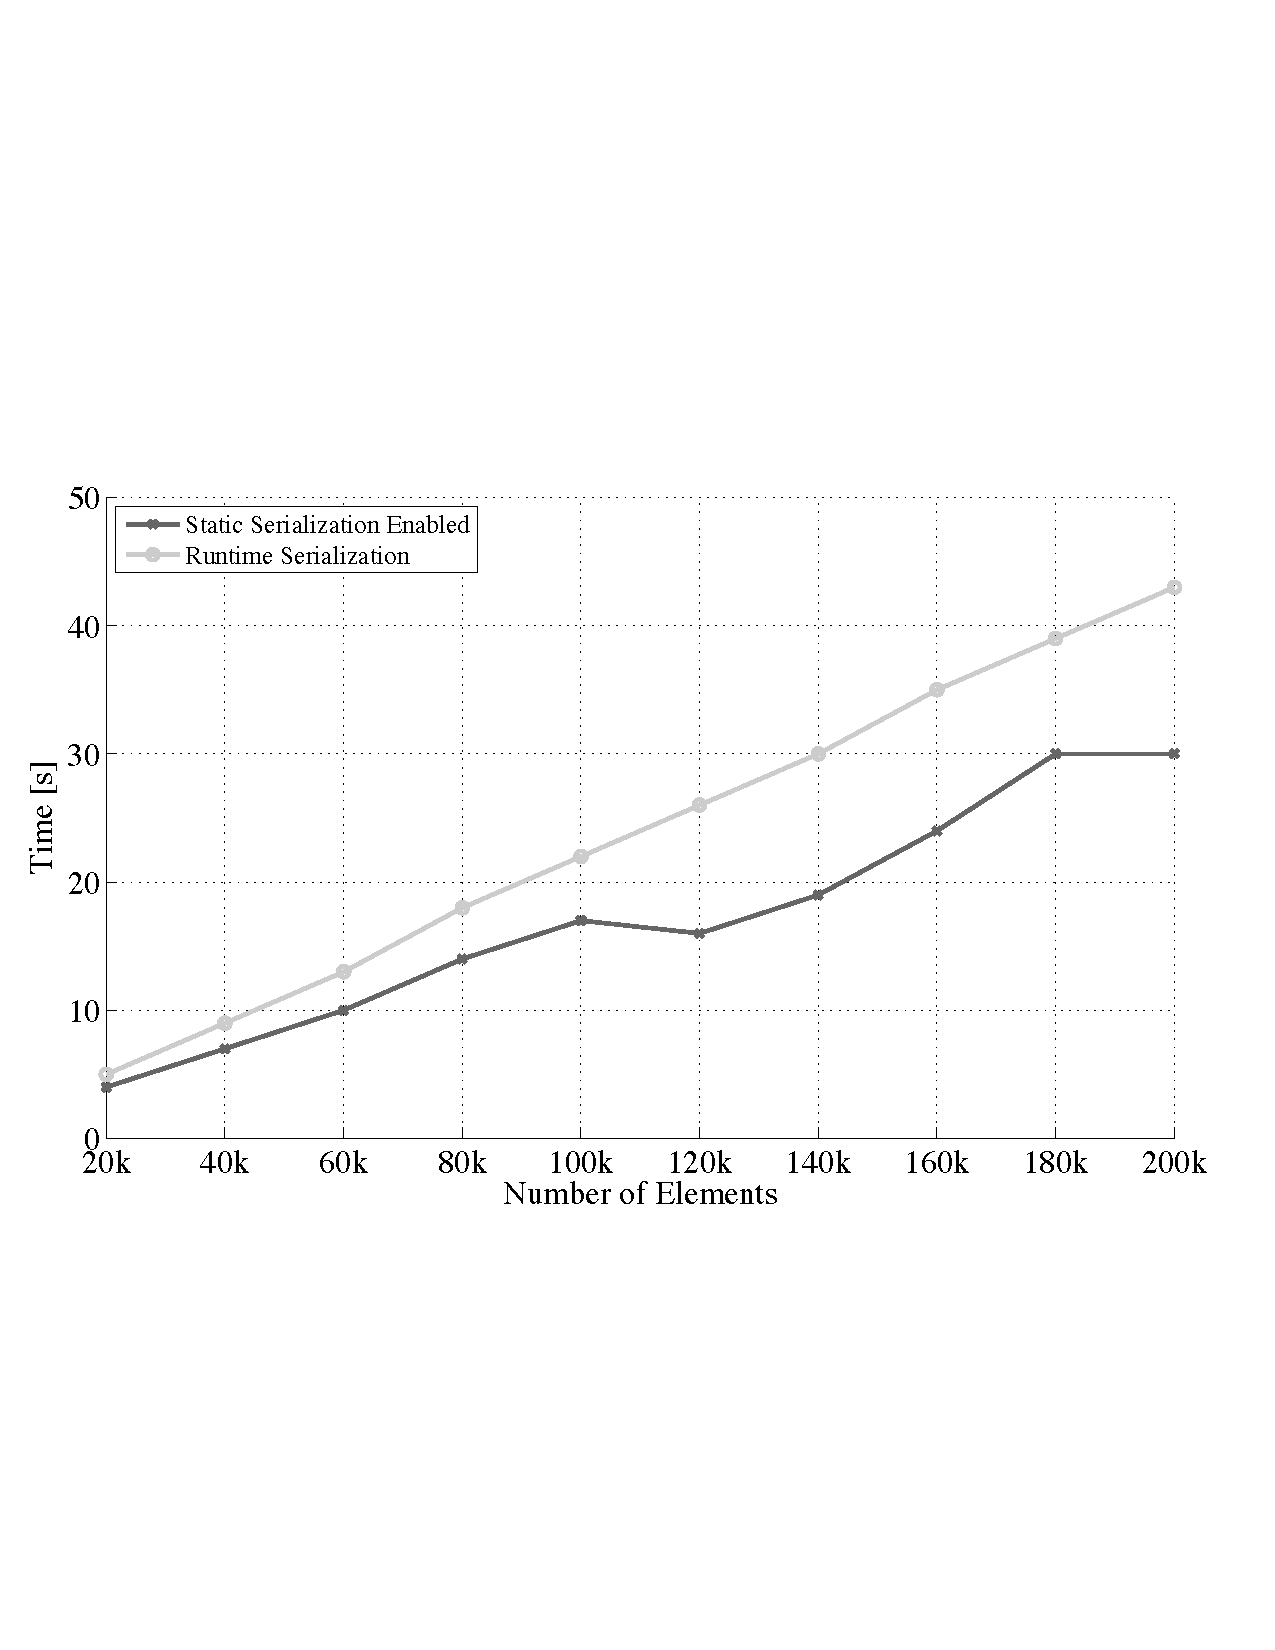
\includegraphics[width=\columnwidth]{multipleJVM.pdf}
% \caption{Impact of Static Types on Performance, End-to-End Application (\texttt{groupBy} + \texttt{join}).}
% \label{fig:multiple-jvm}
% \end{figure}
%
% We have used our implementation to measure the impact of type-specific,
% compile-time-generated serializers (see above) on end-to-end application
% performance. In our benchmark application, a group of 4 silos is distributed
% across 4 different nodes/JVMs. Each silo is populated with a collection of
% ``person'' records. The application first transforms each silo using
% \emph{map}, and then using \emph{groupBy} and \emph{join}. For the benchmark we
% measure the running time for a varying number of records.
%
% We ran our experiments on a 2.3 GHz Intel Core i7 with 16 GB RAM under Mac OS X
% 10.9.5 using Java HotSpot Server 1.8.0-b132. For each input size we report the
% median of 7 runs. Figure~\ref{fig:multiple-jvm} shows the results.
% Interestingly, for an input size of 100,000 records, the use of type-specific
% serializers resulted in an overall speedup of about 48\% with respect to the
% same system using runtime-based serializers.

\section{Examples}
\label{sec:examples}

To show that the function passing model is able to serve as a substrate upon
which to build different sorts of data-centric distributed frameworks, we
provide two miniaturized example systems built on top of F-P that are inspired
by popular big data frameworks; Spark's RDD (Resilient Distributed
Datasets)~\cite{Spark}, and MBrace~\cite{MBrace}. Using each example system,
we've implemented several example applications, excerpts of some of which are
explained below.

Spark's RDDs provide a set of operations to execute parallel operations on
distributed data. MBrace extends F\#’s asynchronous workflows, a way to declare
asynchronous tasks, to distribute computation in the cloud.

Our simplified RDD implementation lets you use data structures distributed
inside Silos using the function passing model. We've implemented some of the
operations of Spark’s RDD such as \verb|map|, \verb|reduce|, \verb|groupBy| and
\verb|join| in terms of the function passing model's primitives. Methods on RDDs
like \verb|flatMap| or \verb|filter| that don’t need to communicate across Silos
are implemented with the function passing model’s \verb|map| using the
corresponding method on the underlying Scala’s collections, while \verb|join| is
implemented using the function passing model’s \verb|flatMap|. Below, we use it
to show a simple application associating the length of all words in two
documents in a \verb|Map| to a set of words with the corresponding length.

\begin{lstlisting}
val content: RDD[String, List[String]] = ...
val lorem: RDD[String, List[String]] = ...

val contentWord = content.flatMap(line => {
  line.split(' ').toList
}).map(word => (word.length, word))

val loremWord = lorem.flatMap(line => {
  line.split(' ').toList
}).map(word => (word.length, word))

val res: Map[Int, Set[String]] =
  contentWord.join[Set, Map](loremWord).collectMap()
\end{lstlisting}

In this example, the closure inside the RDD's \verb|flatMap| method called on
each \verb|contentWord| and \verb|loremWord| splits each line as a list of
words, and flattens everything as a single list. Each word is then mapped to a
tuple containing its length and the word. Finally, we do an inner join, which in
turn associates each length to the set of words of the same length, removing
duplicate words in the process. Finally, we collect the final result in a
\verb|Map| using the \verb|collectMap| method on RDDs. Several other more
detailed example programs using Spark on the function passing model are
available on GitHub.\footnote{\url{https://github.com/Kazy/f-p}}

In the context of MBrace, we also implemented the K-Means Clustering example
available on the MBrace's
website\footnote{\url{http://mbrace.io/starterkit/HandsOnTutorial.FSharp/examples/200-kmeans-clustering-example.html}},
an excerpt of which is shown below. Our implementation of a distributed K-Means
using the function passing model is an almost identical port of the MBrace’s
version written in F\#. K-Means is an algorithm to categorize data points across
$K$ different clusters. It starts with the centroids of the $K$ clusters.

\begin{lstlisting}
def kMeansIterate(
  partitionedPoints: Seq[SiloRef[Array[Point]]],
  centroids: Array[Point],
  iteration: Int): Array[Point] = {

  // Running iteration...
  val clusterParts = partitionedPoints.map(silo => {
    silo.map(spore {
      val lCentroids = centroids
      points => kmeansLocal(points, lCentroids)
    }).send()
  })

  val newCentroids =
    Await.result(Future.sequence(clusterParts).map(seq => {
      seq
        .reduce(_ ++ _)
        .groupBy(_._1)
        .toSeq
        .sortBy(_._1)
        .map(_._2)
        .map(clp => clp.map(_._2).toArray.unzip)
        .map({ case (ns, points) => ns.sum -> sumPoints(points) })
        .map({ case (n, sum) => divPoint(sum, n) })
    }), 10.seconds).toArray

  val diff = newCentroids
    .zip(centroids)
    .map({ case (p1, p2) => dist(p1, p2) })
    .max

  // check if converged, else iterate again
  if (diff < epsilon) {
    newCentroids
  } else {
    kMeansIterate(partitionedPoints, newCentroids, iteration + 1)
  }
}
\end{lstlisting}

The algorithm proceeds with two steps. It first assigns data points to the
closest cluster. Then it assigns to each cluster a new centroid by computing the
mean of the points assigned to the clusters. It stops when the centroids stop
changing; if this convergence condition hasn't been met, the algorithm is called
recursively with the updated set of centroids. In the distributed version of
K-Means, we start with a master node that partitions the points into silos. At
each iteration, \verb|map| is called on the SiloRef which results in a spore
(function) being applied to the data within the corresponding silo. The spore
captures the current iterations' centroids and uses them to compute the new
cluster for its local set of points (using the \verb|kmeansLocal| function). The
results are then sent back to the master node to compute the new centroids, and
to verify the algorithm's convergence condition.






% \section{Evaluation}
% \label{sec:evaluation}

% We provide a small evaluation of our implementation to demonstrate the
% practical benefit of some of the design points of our model.

\section{Related Work}
\label{sec:related-work}

Alice ML~\cite{AliceML} is an extension of Standard ML which adds a number of
important features for distributed programming such as futures and proxies. The
design leading up to the function passing model has incorporated many similar
ideas, such as {type-safe}, generic and platform-independent pickling. In Alice,
functions intend to be mobile. Only those functions which capture (either
directly or indirectly) local resources remain stationary. In the case of
functions that must remain stationary, it is possible to send proxies, mobile
wrappers for functions. Sending a proxy will not transfer the wrapped function;
instead, when a proxy function is applied, the call is forwarded by the system
to the original site as a remote invocation (pickling arguments and result
appropriately). In F-P, however, functions are not wrapped in proxies but sent
directly. Thus, calling a received function will not lead to remote invocations.

Cloud Haskell~\cite{CloudHaskell} leverages guaranteed-serializable, static
closures for a message-passing communication model inspired by Erlang. In
contrast, in our model spores are sent between passive, persistent silos. 
Moreover, the coordination of concurrent activity is based on futures, instead
of message passing. Closures and continuations in Termite
Scheme~\cite{TermiteScheme} are always serializable; references to non-serializable
objects (like open files) are automatically wrapped in processes
that are serialized as their process ID. Similar to Cloud Haskell, Termite is
inspired by Erlang. In contrast to Termite, the function passing model is statically typed, enabling
advanced type-based optimizations. In non-process-oriented models, parallel
closures~\cite{ParallelClosures} and RiverTrail~\cite{RiverTrail} address
important safety issues of closures in a concurrent setting. However,
RiverTrail currently does not support capturing variables in closures, which is
critical for the flatMap combinator in the function passing model. In contrast to parallel closures,
spores do not require a type system extension in Scala.

Acute ML~\cite{AcuteML} is a dialect of ML which proposes numerous primitives
for distributed programming, such as type-safe serialization, dynamic linking
and rebinding, and versioning. The function passing model, in contrast, is based on spores, which ship
with their serialized environment or they fail to compile, obviating the need
for dynamic rebinding. HashCaml~\cite{DistOCaml} is a practical evolution of
Acute ML's ideas in the form of an extension to the OCaml bytecode compiler,
which focuses on type-safe serialization and providing globally meaningful type
names. In contrast, function passing is merely a programming model, which does not require
extensions to the Scala compiler.

% compiler, which focuses on transmitting safe functions to work on remote
% distributed data.

ML5~\cite{Tom7} provides mobile closures verified not to use resources not
present on machines where they are applied. This property is enforced
transitively (for all values reachable from captured values), which is stronger
than what plain spores provide. However, type constraints allow spores to
require properties not limited to mobility. Transitive properties are supported
either using type constraints based on type classes which enforce a transitive
property or by integrating with type systems that enforce transitive
properties. Unlike ML5, spores do not require a type system extension. Further,
the function passing model sits on top of these primitives to provide a full programming
model for distribution, which also integrates spores and type-safe pickling.

% However, type constraints allow spores to require properties not limited to
% mobility. Transitive prop- erties are supported either using type constraints
% based on type classes which enforce a transitive property or by integrating
% with type systems that enforce transitive properties. Unlike ML5, spores do
% not require a type system extension.

Systems like Spark~\cite{Spark}, MapReduce~\cite{MapReduce}, and
Dryad~\cite{Dryad} are just that--distributed systems. The function passing model is meant to act as
more of a middleware to facilitate the design and implementation of such
systems, and as a result provides much finer-grained control over details such
as fault handling and network topology (\ie peer-to-peer vs master/worker).

The Clojure programming language proposes agents~\cite{Clojure}--stationary
mutable data containers that users apply functions to in order to update an
agent's state. The function passing model, in contrast, proposes that data in stationary containers be
immutable, and that transformations by function application form a persistent
data structure. Further, Clojure's agents are designed to manage state in a
shared memory scenario, whereas the function passing model is designed with remote references for a
distributed scenario.

The function passing model is also related to the actor model of concurrency~\cite{Actors},
which features multiple implementations in
Scala~\cite{ScalaActors,Akka,TypedActors}. Actors can serve as in-memory data
containers in a distributed system, like our silos. Unlike silos, actors
encapsulate behavior in addition to immutable or mutable values. While only
some actor implementations support mobile actors (none in Scala), mobile
behavior in the form of serializable closures is central to the function passing model.

% Session
% Types~\cite{SessionTypes}. AmbientTalk~\cite{AmbientTalk}. E
% Language~\cite{ELang}.

% Other clean slate language designs have been proposed to broadly address
% issues related to distributed programming. Thorn~\cite{Thorn} was designed
% with concurrency and the need to interact with remote services in mind. Though
% a main design goal of Thorn is to evolve scripts into typed programs via
% gradual typing. function passing on the other hand is not a language, but a programming
% model, which is designed to inject types into distributed programs from the
% get-go.

% function passing integrates a distributed, persistent data structure. Other prior work
% related to spores is discussed in~\cite{Spores}.

% Type-safe distributed programming in ML5~\cite{Tom7} introduces a notion of a
% typed context called a ``world'' and permits functions to be executed given a
% specific world.

\section{Future Work and Conclusion}
\label{sec:conclusion-future-work}

\subsection{Ongoing and Future Work}

In ongoing work we are exploring approaches for memory reclamation. The first
approach uses Java's WeakReferences to detect when a SiloRef is no longer
reachable from local GC roots. Upon detection the host of the corresponding silo
is notified to decrease the silo's reference count; the host's reference(s) to
the silo are nulled out when the reference count reaches zero. It is important
to note that this strategy requires notifying a silo's host whenever a SiloRef
to the silo reaches a new machine, to increase the silo's reference count. The
second approach leverages uniqueness types in Scala~\cite{Haller10,Haller16}.
Here, SiloRefs are locally unique, and the programmer can explicitly declare a
SiloRef as unused (or ``consumed''); the type system ensures that such an
``unused'' SiloRef is not used
again subsequently. As in the first approach, upon marking a SiloRef as unused,
the corresponding silo's host is notified to decrease the silo's reference
count.

Other future work includes better understanding concerns of separate compilation
in order to evaluate whether our model could be of help in coordinating between
microservices.\footnote{Microservices are small, independent
(separately-compiled) services running on different machines which communicate
with each other to together make up a single and complex application. They are a
predominant trend in industry amongst rich and complicated web-based services.}

\subsection{Conclusion}

We have presented the function passing model, a new programming model and new
substrate or middleware upon which to build data-centric distributed systems.
This enables two important benefits for distributed system builders; since (a)
all computations are functional transformations on immutable data,
fault-tolerance is made simple by design, and (b) communication is made
well-typed by design, the function passing model attempts to more naturally
model the paradigm of data-centric programming by extending monadic programming
to the network. One insight of our model is that lineage-based fault recovery
mechanisms, used in widespread frameworks for distribution, can be modeled
elegantly in a functional way using persistent data structures. Our operational
semantics shows that this approach makes it even amenable to formal treatment.
We have also shown that the function passing model is able to express patterns
of computation richer than those supported by common ``big data'' frameworks
while maintaining fault-tolerance--such as decentralized peer-to-peer patterns
of communication. Finally, we have implemented our approach in and for Scala,
and have shown that it's possible to support different popular patterns of
distributed processing, such as  batch processing with Spark's RDDs  and
MBrace's cloud-based asynchronous tasks.

% We have presented the function passing model, a new programming model and new
% substrate or middleware upon which to build data-centric distributed systems.
%
% This enables two important benefits for distributed
% system builders; (a) since all computations are functional transformations on
% immutable data, fault-tolerance is made simple by design, and (b) communication
% is made well-typed by design, a common pain point for builders of distributed
% systems in Scala. Said another way, the function passing model attempts to more
% naturally model the paradigm of data-centric programming by extending monadic
% programming to the network.
%
% This new model is designed to make it easier to reason about One insight of our
% model is that lineage-based fault recovery mechanisms, used in widespread
% frameworks for distribution, can be modeled elegantly in a functional way using
% persistent data structures.
%
% Our operational
% semantics shows that this approach makes it even amenable to formal treatment.
%
% We have also shown that the function passing model is able to express patterns of computation richer
% than those supported by common ``big data'' frameworks while maintaining
% fault-tolerance--such as decentralized peer-to-peer patterns of communication.
%
% Finally, we have implemented our approach in and for Scala, as well as numerous
% applications on top. We've shown
%
% , and have discovered new ways to reconcile type-specific
% serializers with patterns of static typing common in distributed systems.



% We have presented the function passing model, a new programming model and principled substrate for
% building data-centric distributed systems. Built atop a foundation consisting
% of performant and type-safe serialization, and safe, serializable closures, we
% have shown that it's possible to build elegant fault-tolerant functional
% systems. One insight of our model is that lineage-based fault recovery
% mechanisms, used in widespread frameworks for distribution, can be modeled
% elegantly in a functional way using persistent data structures. Our operational
% semantics shows that this approach makes it even amenable to formal treatment.
% We have also shown that the function passing model is able to express patterns of computation richer
% than those supported by common ``big data'' frameworks while maintaining
% fault-tolerance--such as decentralized peer-to-peer patterns of communication.
% Finally, we have implemented our approach in and for Scala, as well as numerous
% applications on top, and have discovered new ways to reconcile type-specific
% serializers with patterns of static typing common in distributed systems.
%
% A great deal of future work remains. In the short-term, we aim to continue to
% build different sorts of distributed frameworks and applications atop the function passing model in an
% effort to work towards a production-ready implementation of our model for
% consumption by the Scala community at large.

% Adapt this model for streaming computation. This would take coming up with a
% solution to null out references in the {\em lineage}. This would make it
% possible to instantiate and populate new silos to handle incoming data.

% The most successful systems for ``big data'' processing have all adopted
% functional APIs. But the innards of these systems are often built atop
% imperative and weakly-typed stacks, which complicates the design and
% implementation of distributed system essentials like fault-tolerance. We
% present a new programming model we call  {\em function passing} designed to
% overcome many of these issues by providing a more principled substrate on
% which to build data-centric distributed systems. A key idea is to pass safe,
% well-typed serializable functions to immutable distributed data.  The function passing
% model itself can be thought of as a distributed persistent functional data
% structure, which stores in its nodes transformations to data rather than the
% distributed data itself.  Thus, the model simplifies failure recovery by
% design--data is recovered by replaying function applications atop immutable
% data loaded from stable storage. Lazy evaluation is also central to our
% model; by carefully incorporating laziness into our design (only at the point
% of initiating network communication), our model remains easy to reason about
% while remaining efficient in time and memory. We formalize our programming
% model in the form of a small-step operational semantics which includes a
% precise specification of the semantics of functional fault recovery. We
% implement our model in and for the Scala programming language, and provide a
% small evaluation of the efficiency of our implementation of the model.

% \section{Future Work}

% Adapt this model for streaming computation. This would take coming up with a
% solution to null out references in the {\em lineage}. This would make it
% possible to instantiate and populate new silos to handle incoming data.

% \section{Old}

% \subsection{Old Intro}

% % From the ivory tower, it may not be evident,
% % It might not seem this way from the ivory tower,
% % but

% While it might not seem that way at a glance, mainstream software development
% has become largely distributed. Two {\em styles} of distribution dominate the
% current landscape; (1) systems composed of microservices, % or designed to be
% software as a service (SaaS), and (2) systems for ``big data'' processing.
% Names like Netflix, SoundCloud, and Twitter have established their
% competitive offerings by way of one or both of these types of systems.

% Microservices are small, independent (separately-compiled) services running
% on different machines which communicate with each other to together make up a
% single and complex application. ``Big data''-style applications on the other
% hand are typically single applications whose data cannot fit into the memory
% of one machine alone. Such applications are typically singly-compiled, with
% their binaries distributed across a cluster of machines.

% Yet, software developers still fumble with low-level RPC frameworks.  % and
% sluggish serialization frameworks.  Mainstream programming languages have
% traditionally offered little support in this space.

% We design module systems, etc, for maximum reuse and productivity, we go as
% far as we can to demonstrate their power. But we often . Some of these
% concerns have been affectionately referred to as the ``awkward
% squad''~\cite{AwkwardSquad} by PL research, and they are concerns that are
% central to contemporary software development.

% Functional programming brings value to distributed systems builders. The
% success of popular Spark can be attributed to functional ideas.

% However, beyond Spark's interface, .

% We refer to the model as {\em function-passing}, and .

% We design a programming model in such a way that we can ``maximize'' static
% types, and with it enable type-specialized picklers (statically generated),
% typed closures, and type-specialized data structures.

% The motto is ``making type inference work for you when optimizing distributed
% systems'', or ``how type inference and existential types benefit distributed
% systems''.

% In existing systems, types are only in the user-facing API and help the user.
% However, all too often, the internals of a distributed system are largely
% untyped, in particular when operating on data types that are also shipped
% remotely. In our approach we now go ahead and make types work so that they
% benefit both users (helping catch common errors) \emph{and} distributed
% systems builders. Our approach leverages types to provide (1)
% type-specialized picklers, and (2) type-specialized collections/builders.

% The approach is novel, because noone talks about making sure the unpicklers
% and builders themselves are serializable, but that's actually fundamental to
% the whole design.

% \begin{itemize}

% \item We have to make the point that serialization is like a primitive in
% systems design, not some extra thing you figure out how to do later, like in
% typical PLs. so maybe one central point that we should try to make is that
% for distributed systems, serializability is like a key primitive, along with
% latency and other things.

% \item we want to prove that typed distributed systems are a good idea. right
% now a lot of systems for dist computing are fundamentally untyped or
% dynamically checked. those that are typed lose type information between
% machines.

% \item so we're trying to argue that types are good for system builders.

% \end{itemize}

% The fact that actually these benefits from types \emph{carry over to other
% models as well} (not just spark-like models).

% Generalization of MapReduce model. Low-level. Inversion of the actor model.
% Can represent different many models for distributed computing, e.g. Spark,
% Percolator (we probably can't validate this claim.)

% Illustrations to have:
% \begin{enumerate}
% \item nice figure
% \item organic evolving model on youtube
% \end{enumerate}

% \subsection{Evaluation}

% we could make the performance eval strong by saying, ok, we implemented real
% apps, so we have the real communication that needs to happen (and happens).
% and we now make this communication typed, plus we measure exactly the
% percentage of time that's spent in serialization for example. and then we
% could even interpolate the results, so we could say, ok, if some other dist
% system has a lower percentage spent in serialization, then the speed up would
% be like this.

% and then we could even measure that for real spark, and then interpolate and
% say, ok, in the ideal case, meaning using all of our design principles, we
% could speed up things like this, if one would re-architect spark to preserve
% types (it's a huge task, so out of scope).

% well, it would definitely be something that we can measure objectively. the
% only thing we have to guard against would be to say, adding picklers and
% builders does not otherwise \emph{degrade} performance, like, we'd have to
% prove that there's no cost, but \emph{just} the performance benefits. adding
% the classname of the unpickler adds a few bytes to each pickle, for example.

% we could even show that with babyspark, like have a version that uses java
% serialization, then a version that uses pickling without selfdescribing, then
% with runtime unpickling, and with all static. because we have those numbers
% for babyspark then the interpolation will be much more precise.

%%%%%%%%%%%%%%%%%%%%%%%%%%%%%%%%%%%%%%%%%%%%%%%%%%%%%%%%%%%%%%%%%%%%%%%%%%%%
%\appendix
%\section{Appendix Title}
%
%This is the text of the appendix, if you need one.
%
%\acks
%
%Acknowledgments, if needed.

% We recommend abbrvnat bibliography style.

\bibliographystyle{abbrvnat}
\balance
\bibliography{bib}

% The bibliography should be embedded for final submission.
%\begin{thebibliography}{}
%\softraggedright
%
%\bibitem[Smith et~al.(2009)Smith, Jones]{smith02}
%P. Q. Smith, and X. Y. Jones. ...reference text...
%
%\end{thebibliography}

\end{document}
